% !TEX root = ./main.tex

%%% Setup Page Layout

\documentclass[
	paper=a4,
	fontsize=12pt,
	BCOR=5mm,
%	openany,
	headinclude,
	% fontinclude=true,
%	cleardoublepage=empty,
	pagesize=pdftex,
	headsepline,							% Line under page header
	%footsepline,
	%toc=bib, index=totoc,
	toc=listof,
	%report,
	toc=bibliography,
	% setcapindent,
	% titlepage=true,
	english
]{scrreprt}

\usepackage[onehalfspacing]{setspace}	% Should set up onehalfspacing, copied from Steffen
% \setlength{\parskip}{0.5cm plus0.2cm minus 0.2cm}

%%% Setup Encoding and Fonts

\usepackage[utf8]{inputenx}
\usepackage[T1]{fontenc}
\usepackage{lmodern}
% Somehow, lmodern has to be loaded before mathdesign. Otherwise, the font looks like garbage
\usepackage[bitstream-charter]{mathdesign}	% Charter-BT Font
%\let\circledS\undefined		% suppress error of multiply defined \circledS
% \usepackage{amssymb}
%\usepackage{mdbch}

%%% Setup Document Language

\usepackage[english]{babel}

%%% Setup Graphics

\usepackage{graphicx}
\usepackage{subcaption}
	\graphicspath{ {images/} }

% Used to outsource tikz code and include it in a figure environment
\usepackage{standalone}
\usepackage{tikz}
\usetikzlibrary{shapes,arrows}

%%% Setup Headers and Footers

\usepackage{scrlayer-scrpage}		% Part of KOMA-Script, formatting headers and footers
\clearscrheadfoot				% remove standard head- and footline
\automark*{chapter}				% redefine chapter style
\ohead*{\pagemark}				% Sets pagenumber on outer headline, including chapterpage
\ihead{\headmark}				% Sets current section on inner headline, excluding chapterpage

%%% Setup Tables

\usepackage{tabularx}					% https://www.ctan.org/pkg/tabularx page wide tables
\usepackage{multirow}					% https://www.ctan.org/pkg/multirow
\usepackage{booktabs}					% https://www.ctan.org/pkg/booktabs nicer tables
\usepackage{float}						% https://www.ctan.org/pkg/float
\usepackage{longtable}					% https://ctan.org/pkg/longtable tables spanning more than one page

\usepackage[
	justification=RaggedRight,
	singlelinecheck=false
]{caption}

%%% Setup Bibliography

\usepackage{csquotes}					% https://www.ctan.org/pkg/csquotes required for biblatex
\usepackage[							% https://www.ctan.org/pkg/biblatex
	style=chem-acs,						% American chemical society citation style
	autocite=superscript				% Sets numbers in superscript
]{biblatex}
\addbibresource{references/library.bib}	% Bibliography location

%%% Misc. Packages

\usepackage{siunitx}					% Formatting SI units
	\sisetup{detect-all}				% Changes SI-number font to global font
\usepackage{chemformula}				% Formatting chemical elements
\usepackage{microtype}					% khirevich.com/latex/microtype
\usepackage{pdfpages}					% Include titlepage as pdf
\usepackage{scrhack}					% Removes Errors from Koma-Script Packages
\usepackage{todonotes}					% Adds Todo-Notes
\usepackage{textgreek}					% Allow greek letters without math mode


%%% Custom Comands

% Shortcuts for species names
\newcommand{\coli}{\textit{E. coli}~K12}		
\newcommand{\bac}{\textit{B. subtilis}~168}
\newcommand{\tue}{\textit{Streptomyces}~sp.~Tü2401}

% Shortcuts for columns
\newcommand{\luna}{Luna\textsuperscript{\textregistered} NH\textsubscript{2}}

% Other Shortcuts
\newcommand{\pka}{p\textit{K}\textsubscript{a}}

\begin{document}

% 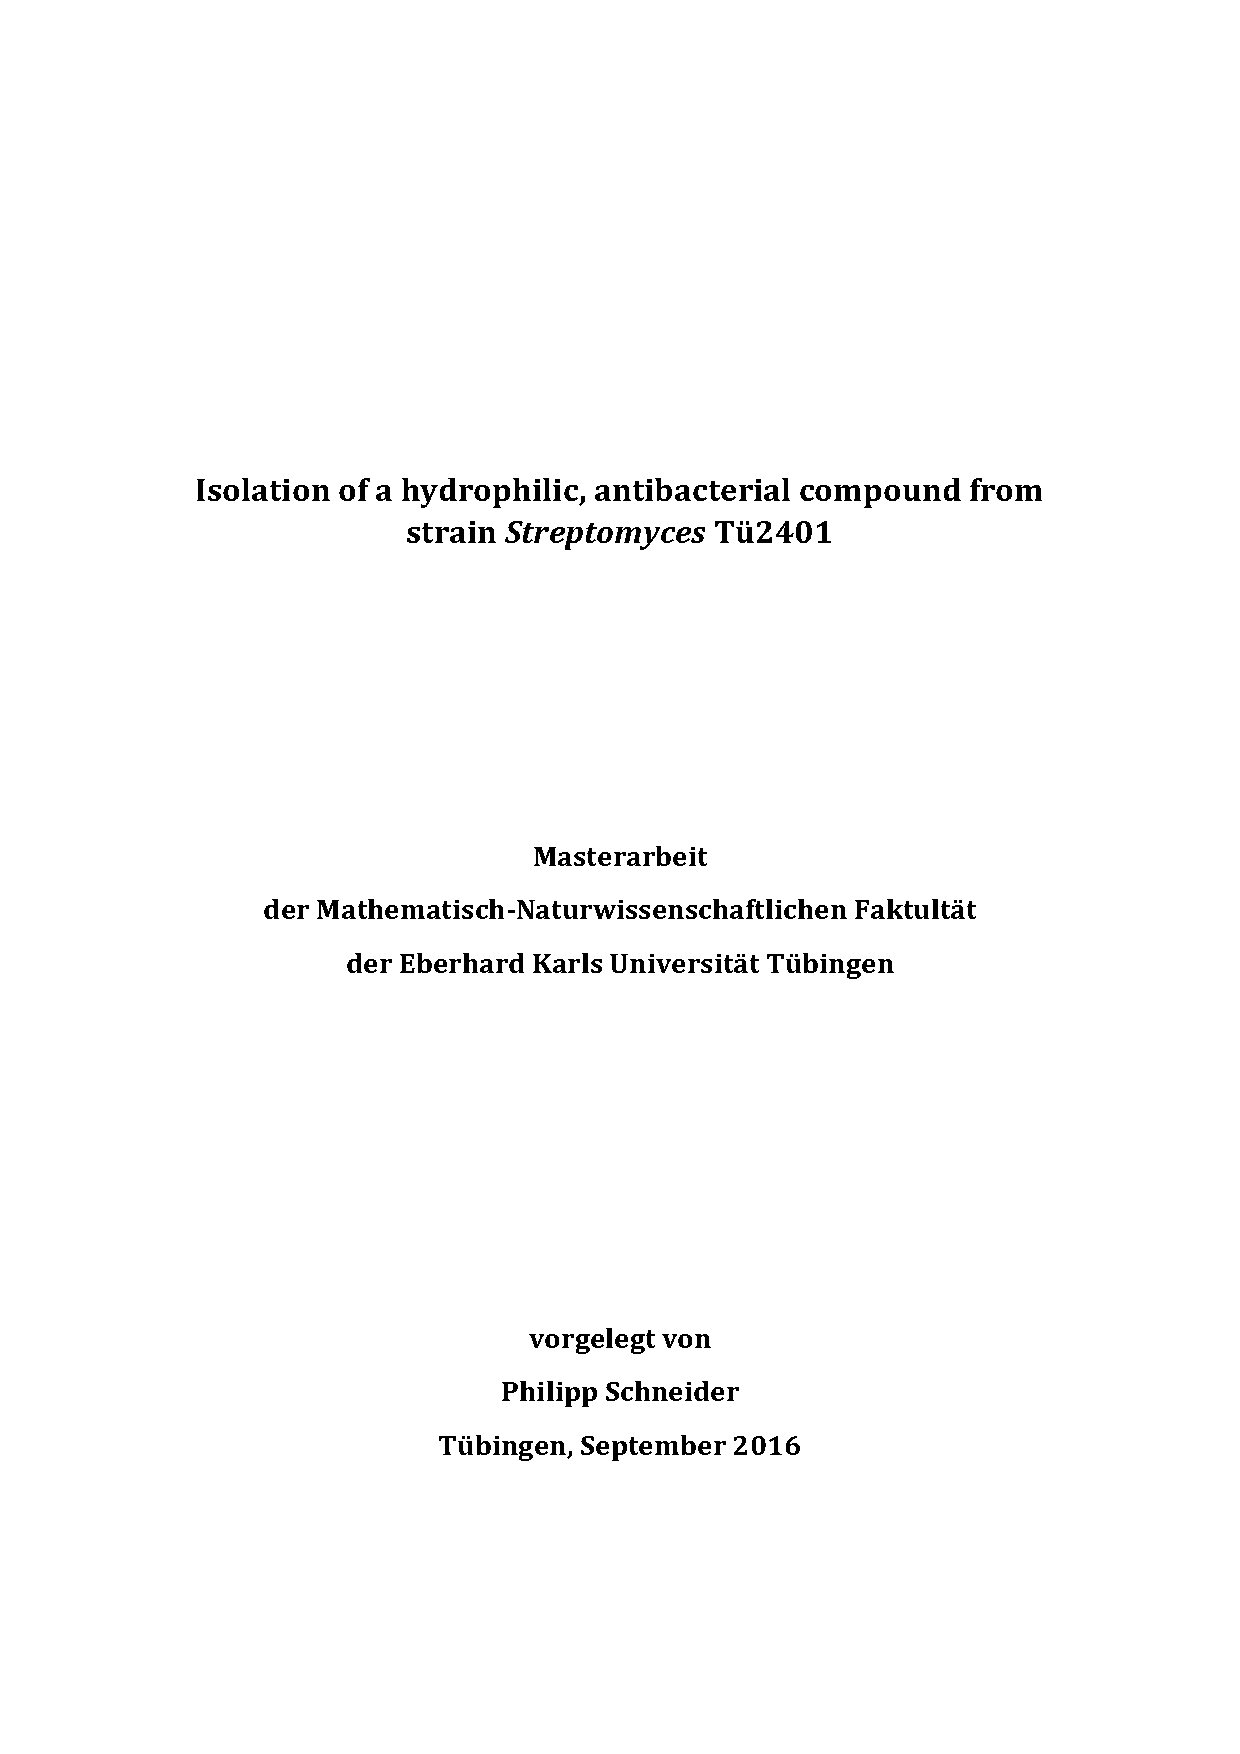
\includepdf{testtitle}

% \titlehead{{\Large Eberhard-Karls-Universit\"at T\"ubingen
% 	\hfill WS2017\\}
% 	Mathematisch-Naturwissenschaftliche Fakult\"at\\
% 	Auf der Morgenstelle~28\\
% 	72071 T\"ubingen}% \subject{Masterarbeit}
% \title{Isolation of antibacterial natural products from \textit{Streptomyces} sp. Tü2401}
% \author{Philipp Schneider}
% \date{1. November 2017}
% \publishers{Betreut durch Prof. Dr. Timo Niedermeyer}
% \maketitle


% \addchap*{Erkl\"arung}

% Hiermit erkl\"are ich,
% \\
% \\
% - dass ich diese Arbeit selbst verfasst habe.
% \\
% \\
% - dass ich keine anderen als die angegebenen Quellen benutzt und dass ich alle wörtlich oder sinngemäß aus anderen Werken \"ubernommenen Aussagen als solche gekennzeichnet habe.
% \\
% - dass die eingereichte Arbeit weder vollst\"andig noch in wesentlichen Teilen Gegenstand eines anderen Pr\"ufungsverfahrens gewesen ist.

% \newpage

% \addchap*{Zusammenfassung}

\addchap*{Abstract}
The strain \textit{Streptomyces} sp. Tü2401 is capable of producing antimicrobial compounds which are active against diverse types of bacteria. Preliminary screening showed potent activity against several multiresistant \textit{Escherichia coli} strains as well as the Gram-positive strains \textit{Bacillus subtilis} and \textit{Staphylococcus aureus}. Additionally, a mode-of-action \textit{Bacillus} reporter strain indicated the presence of substances, which inhibit DNA synthesis. The broad activity spectrum and the unusual mode of action make this strain a valuable target of bioactivity-guided isolation of its natural products.

The

% \addchap*{Danksagung}
% % I want to thank...

% \pagenumbering{Roman}

\tableofcontents
% \listoffigures
% \listoftables

% \addchap*{Abbreviations}
% % !TEX root = ../main.tex
\addchap{Abbreviations}

\begin{table}[htbp]
	\centering
	\begin{tabularx}{\textwidth}{>{\hsize=0.25\hsize}X>{\hsize=0.75\hsize}X}
		\toprule
%		\textbf{Abbreviation}		& \textbf{Description}			\\
%		\midrule
		AntiSMASH	& Antibiotics \& Secondary Metabolites Analysis Shell	\\
		EtAc		& Ethyl acetate			\\
		EtForm		& Ethyl formate			\\
		GC			& Gas Chromatography	\\
		MeAc		& Methyl acetate		\\
		MS			& Mass Spectrometry		\\
		HPLC		& High Performance Liquid Chromatography		\\
		OD\textsubscript{600}	& Optical Density at \SI{600}{\nano\meter}	\\
		TLC			& Thin Layer Chromatography 	\\
		TMS 		& Trimethylsilane		\\
		Tü2401		& \textit{Streptomyces} sp. Tü2401		\\
		
		
		\bottomrule
	\end{tabularx}
\end{table}


% \clearpage
% \pagenumbering{arabic}

% \chapter{Introduction}
% % !TEX root = ../main.tex

\section{First part} % (fold)
\label{sec:first_part}



Lorem ipsum dolor sit amet, consectetur adipiscing elit. Fusce hendrerit efficitur orci id sodales. Nulla euismod sapien at velit efficitur, in interdum nunc pulvinar. Aenean tempor quis enim ut varius. Suspendisse pellentesque tincidunt elit, eget placerat nisl tempus non. Maecenas eget odio est. Maecenas in quam ut felis varius molestie. Donec porta eros nec leo egestas lacinia. Duis venenatis nulla lacus.

Vestibulum pretium porta nunc, ut rhoncus massa dapibus at. Duis in velit aliquam, malesuada lectus id, posuere leo. Integer malesuada sem sit amet turpis cursus vestibulum. Fusce nec libero in massa congue volutpat sit amet nec felis. Etiam pellentesque tortor at mattis lacinia. Duis sit amet mollis turpis, nec convallis tortor. Nullam quis quam lacinia, vulputate nisl id, rhoncus mi. Morbi congue, massa et elementum aliquet, odio tellus mollis nulla, eu aliquam risus est et erat. Nunc non leo arcu. Curabitur id congue ligula, sit amet imperdiet quam. Duis cursus urna nec sagittis cursus. In ac consectetur justo. Praesent tortor est, bibendum a porttitor sed, ultricies id dui. Praesent hendrerit nibh in posuere iaculis. Ut sed neque id leo luctus laoreet non ut quam.

Aliquam quis consectetur augue, ac commodo erat. Integer sed sapien nec dui dictum mattis. Duis sapien risus, consectetur vel velit ac, aliquet ultricies nunc. Curabitur sit amet ligula id odio pharetra suscipit et sit amet purus. Maecenas a malesuada nunc. Cras sed libero nisl. Sed gravida sed justo sed pulvinar. Vestibulum a maximus neque. Donec nec leo vel nibh euismod porttitor. Nullam tortor ex, vehicula convallis massa id, pharetra dignissim est. Proin bibendum nunc ut egestas ullamcorper. Nunc et ornare erat. Sed posuere purus non eros rutrum mattis.

\begin{figure}[htbp]
	\centering
	\begin{subfigure}[b]{0.5\textwidth}
		\centering
		\includegraphics[width=\textwidth]{IMG_9701}
		\caption{Plate 1}
		\label{fig:p1}
	\end{subfigure}% Don't forget this fucking percent! Otherwise it won't be side by side
	\hfill
	\begin{subfigure}[b]{0.5\textwidth}
		\centering
		\includegraphics[width=\textwidth]{IMG_9702}
		\caption{Plate 2}
		\label{fig:p2}
	\end{subfigure}
	\caption{Plate assay of HILIC fractions against K12. asdöjj ösdj sdjkfj  sfsdö sjjfkdjf lskfjsd öaskjös s djfkd s ls s kj sdkjfksjf   als slkd s}
	\label{fig:hilic_ass}
\end{figure}

Sed elit risus, interdum eget velit et, dignissim blandit nibh. Donec eu purus eu justo convallis accumsan. Etiam commodo venenatis libero, in mattis mauris blandit at. Fusce dignissim cursus massa id maximus. Praesent interdum risus et felis aliquet commodo. Duis dapibus sagittis sapien, id vehicula massa consequat a. Aenean sed felis a lectus mollis feugiat. Proin a lorem dictum, tempor augue ut, porttitor erat. Phasellus sed turpis id orci ultrices consequat efficitur et est. Quisque dignissim velit tellus. Duis ut nisi cursus, tincidunt nisi nec, sollicitudin dui. Nulla semper vitae mauris placerat scelerisque. Maecenas euismod a tellus ac pellentesque. Nunc ut justo dolor. Donec posuere sed justo a rhoncus. Nullam ac lacus sodales, bibendum nunc sit amet, tincidunt lorem.

Donec vitae tortor a felis dapibus suscipit ut ut sapien. Cras eleifend purus neque, a auctor dui efficitur id. Curabitur convallis in eros vitae venenatis. Cras ligula ligula, vulputate at purus nec, facilisis hendrerit orci. Curabitur tempus ultrices quam, eu volutpat velit dignissim ac. Orci varius natoque penatibus et magnis dis parturient montes, nascetur ridiculus mus. Curabitur eros velit, sodales sed diam quis, imperdiet blandit orci. Sed convallis sollicitudin felis, ut sagittis ante faucibus ut. Pellentesque facilisis, velit nec ultrices pulvinar, turpis velit lacinia purus, non auctor felis dui vel ligula. Nullam nec tempus elit. Donec consectetur turpis erat, in iaculis risus mollis eget. Donec vulputate, eros in tincidunt iaculis, nisl odio hendrerit mauris, sit amet elementum enim mauris a orci. Proin a diam convallis, dapibus metus in, lacinia sem. Cras commodo molestie ipsum quis feugiat.

In lobortis est eu nulla suscipit facilisis. Proin consequat dapibus auctor. Maecenas nisi ante, convallis non dictum nec, auctor a libero. Quisque iaculis tincidunt nisl sit amet tristique. Suspendisse ultrices tincidunt diam, eget pharetra erat gravida vel. Curabitur sed augue nec mi tempus tempus. Ut viverra lacus nisl, eget tincidunt ipsum iaculis sagittis. Praesent interdum mi quis velit rutrum viverra. Quisque placerat eget magna ut dignissim. Duis finibus malesuada pharetra. Nulla cursus libero a nulla convallis, at iaculis ipsum euismod.

Curabitur euismod ante sed libero pretium bibendum. Nunc vestibulum est non finibus pellentesque. Etiam nec elit in nulla mollis placerat. Nullam sit amet vehicula leo, finibus semper ante. Vestibulum ante ipsum primis in faucibus orci luctus et ultrices posuere cubilia Curae; Curabitur nulla erat, consequat vel dolor luctus, tristique ultrices velit. Integer consequat justo iaculis tortor semper, vitae bibendum velit commodo. Proin in molestie odio. Cras eget justo urna. Etiam porttitor, quam ac consectetur sodales, ante sem dictum magna, id ullamcorper orci nunc at sem. In hac habitasse platea dictumst. Mauris sed justo eu ante facilisis tincidunt. Sed placerat velit et risus congue volutpat a sed ipsum. Aliquam fermentum nulla congue dui imperdiet, quis accumsan magna posuere. Vivamus laoreet arcu ut felis blandit imperdiet.

Etiam egestas magna a odio tincidunt venenatis. Nullam fermentum nisl et est fringilla ullamcorper. Duis vulputate condimentum enim vel pulvinar. Mauris tristique id mi sit amet molestie. Ut auctor et diam ac egestas. Sed augue tellus, vestibulum id massa in, maximus eleifend tellus. Nullam laoreet ex vitae gravida tempus. Fusce tempus pretium quam pulvinar commodo. Nulla lobortis iaculis placerat. Pellentesque arcu purus, ornare id mollis at, sollicitudin non elit. Suspendisse rutrum mi a neque dictum eleifend at sed lorem. Aenean ornare at sem ac cursus. Vivamus sit amet ante luctus orci venenatis imperdiet eu vitae enim. Curabitur varius fermentum dui, sed lacinia nulla euismod eu.

Suspendisse euismod id velit vitae hendrerit. Vestibulum vel lectus sit amet ante iaculis euismod. Vestibulum ullamcorper quis neque id varius. Quisque eget ipsum arcu. Integer et nisi eu ante ultrices semper id vel metus. In hac habitasse platea dictumst. Fusce eu leo euismod, consectetur augue aliquam, egestas risus. Ut vel aliquam dui. Aliquam ullamcorper felis ligula, quis semper arcu semper sit amet.

Duis interdum pulvinar lacus. Suspendisse eget tellus eget urna fermentum porttitor et non massa. Cras euismod suscipit massa quis fringilla. Ut dictum aliquet est. Nunc ac tincidunt tortor, id molestie turpis. Sed tristique, metus sed hendrerit porttitor, lorem nibh molestie lacus, vel scelerisque nibh dolor finibus lorem. Donec suscipit nunc arcu, et ultricies sem consequat vitae. Sed purus ipsum, hendrerit non odio ut, rhoncus aliquam ligula. Sed dui neque, rhoncus nec maximus a, auctor et lectus.

Donec et sollicitudin sem. Aenean aliquet magna sed nisi tristique, sit amet rhoncus elit consequat. Nam euismod enim quam, non placerat eros ultricies eu. Vivamus luctus ultricies neque vitae ornare. Aliquam turpis magna, cursus vel ornare at, egestas vel metus. Vivamus et eros iaculis massa blandit egestas et eu ante. Mauris non aliquam ipsum, eget fringilla velit. Nullam molestie erat velit, nec consequat risus varius in. Pellentesque euismod arcu et lectus aliquam, eu dapibus metus dapibus.

Vestibulum et vulputate risus. Curabitur volutpat arcu eget nunc elementum, a porta sem iaculis. Nunc in leo non dolor dignissim consectetur. Mauris dignissim scelerisque diam, non posuere sem vulputate non. Nullam sagittis condimentum sapien pellentesque gravida. Nam dignissim sapien at nibh faucibus maximus in ac est. Ut id lobortis tortor, in tristique nunc. Proin id odio urna. In leo mi, scelerisque nec ligula in, scelerisque mattis massa. Pellentesque porttitor feugiat nisl tincidunt porta. Fusce sagittis vehicula neque, in bibendum lorem aliquet ut. Sed mollis in risus quis pharetra. Maecenas vulputate sed dolor ac pellentesque. Vivamus vel tincidunt ligula, sed facilisis eros. Duis vulputate tortor ut nibh efficitur, at ullamcorper elit ultricies.

Donec nec malesuada ante, at mollis lectus. Vivamus maximus elementum dolor ac varius. Donec efficitur mollis laoreet. Maecenas commodo lectus at leo rhoncus, sed egestas justo congue. Proin quis volutpat nulla. Morbi feugiat dictum lacus vitae convallis. Sed sed sapien vel nunc consectetur congue.

Nam ultrices eros vel porta iaculis. Quisque lacus nibh, egestas at lacus at, efficitur vehicula est. Mauris eu lorem sit amet orci volutpat posuere. Nullam sed leo non ante posuere varius. Morbi pulvinar venenatis urna ut gravida. Donec aliquet nec magna ut sollicitudin. Pellentesque fringilla est vitae congue dictum. Vivamus et libero tortor. Ut pellentesque vitae turpis eleifend ultricies.

In hac habitasse platea dictumst. Donec elementum nisl eu ullamcorper accumsan. Vivamus maximus tempor lorem eu posuere. Nulla nec ullamcorper massa. Aliquam in ex vitae nulla blandit dignissim. Ut luctus fringilla lorem, nec imperdiet libero malesuada nec. Pellentesque habitant morbi tristique senectus et netus et malesuada fames ac turpis egestas. Nunc dictum arcu non sapien interdum sollicitudin non id leo.

Mauris condimentum lorem vel mi ultrices, eu condimentum neque rutrum. Duis vestibulum eros nec bibendum venenatis. Proin hendrerit elit nisi, sit amet porta lorem lacinia ut. Curabitur vel lacus vulputate, iaculis mi id, fringilla diam. Sed ultricies leo metus, nec porttitor magna posuere et. Duis id leo nec mauris posuere pharetra vel eget quam. Sed vitae sem blandit, tincidunt velit et, auctor lectus. Proin laoreet at felis vitae dignissim. Praesent vitae aliquet lectus. Praesent congue non turpis sit amet venenatis. Vestibulum sit amet nibh in felis dapibus laoreet. Donec sed justo sit amet dolor cursus molestie.

Duis hendrerit mauris sed nulla commodo, sodales iaculis mi tristique. Donec quis sagittis lorem, nec ultrices mauris. Praesent ornare in quam vel suscipit. Donec sed justo diam. Vivamus iaculis euismod est ac euismod. Sed dictum neque ac varius viverra. Fusce purus dui, cursus sit amet molestie condimentum, malesuada a ligula. Morbi eu convallis neque. Donec ligula nibh, semper non interdum non, lacinia quis dolor. Nam hendrerit quam vel consectetur facilisis. Morbi finibus, arcu vitae vulputate cursus, justo mi condimentum. 
% section first_part (end)

% \clearpage

% \chapter{Methods}
% % !TEX root = ../main.tex

\section{Chemicals \& Instruments} % (fold)
\label{sec:chemicals_&_instruments}

	Chemicals and solvents were supplied by Merck, if not specified otherwise. Differing vendors for solvents are listed in Table~\ref{tab:solvent_table}

	\begin{table}[htbp]
		\caption{Used chemicals and solvents}
		\label{tab:solvent_table}
		\centering
		\begin{tabularx}{\textwidth}{XX}
			\toprule
			\textbf{Chemical}	&	\textbf{Supplier}	\\
			\midrule
			J. T. Baker			&	Acetonitrile		\\
								&	Chloroform			\\
			Alfa Aesar			&	Methyl acetate		\\
			Fisher Chemicals 	&	Ethyl acetate		\\
		\end{tabularx}
	\end{table}

	% The used instruments are listed in in Table~\ref{tab:labins}.

	% \begin{table}[H]
	% 	\caption{Used laboratory Instruments}
	% 	\label{tab:labins}
	% 	\centering
	% 	\begin{tabularx}{\textwidth}{XXX}
	% 		\toprule
	% 		\textbf{Instrument}			& \textbf{Model}		& \textbf{Manufacturer}	\\
	% 		\midrule
	% 		Centrifuges			&	Megafuge 1.0 (R)		&	Heraeus Instruments 	\\
	% 							&	Centrifuge 5417 C 		&	Eppendorf	\\
	% 							&	RC6 Plus Centrifuge 	&	Sorvall	\\
	% 		Lyophilizator		&	LyoVac GT2				&	Leybold \\
	% 		Spectrophotometer	&	BioMate 3S				&	Thermo Fisher \\
	% 		Rotary Evaporator	&	Hei-Vap Precision		&	Heidolph \\
	% 							&	Rotavapor RE + PC 3001 VARIO Pump	&	B\"uchi + vacuubrand \\

	% 		\bottomrule
	% 	\end{tabularx}
	% \end{table}

	High performance liquid chromatography (HPLC) systems were manufactured by Agilent. The components of the HPLC systems are listed in Table~\ref{tab:HPLCtab}.

	\begin{table}[htbp]
		\caption{Components of HPLC systems}
		\label{tab:HPLCtab}
		\centering
		\begin{tabularx}{\textwidth}{XXX}
			\toprule
							& \textbf{Component}		& \textbf{Description}	\\
			\midrule
			Agilent 1100 Series		&	G1322A		&	Degasser			\\
									&	G1311A		&	Quaternary Pump		\\
									&	G1313A		&	Autosampler			\\
									&	G1316A		&	Column Compartment	\\
									&	G1315B		&	Diode Array Detector	\\
			\midrule
			Agilent 1200 Series		&	G1379B		&	Degasser			\\
									&	G1312A		&	Binary Pump			\\
									&	G1367B		&	Autosampler			\\
									&	G1330B		&	Thermostat			\\
									&	G1316A		&	Column Compartment	\\
									&	G1315B		&	Diode Array Detector	\\
			\midrule
			Agilent 1260 Infinity	&	G4225A		&	Degasser			\\
									&	G1312C		&	Binary Pump			\\
									&	G1329B		&	Autosampler			\\
									&	G1330B		&	Thermostat			\\
									&	G1316A		&	Column Compartment	\\
									&	G1315D		&	Diode Array Detector	\\
			\bottomrule
		\end{tabularx}
	\end{table}

	\begin{table}[htbp]
		\caption{Column Parameters}
		\label{tab:column_parameters}
		\centering
			\begin{tabularx}{\textwidth}{XXXX}
			\toprule
			\textbf{Manufacturer} 	& \textbf{Line} 						& \textbf{Type} 					& \textbf{Size} 	\\
			\midrule
			Merck 					& SeQuant\textsuperscript{\textregistered} 		& \mbox{ZIC\textsuperscript{\textregistered}-HILIC} PEEK \SI{3.5}{\micro\meter}					& 150 $\times$ 4.6 mm 	\\
			Phenomenex 				& Luna\textsuperscript{\textregistered} 			& NH2 5u		& 250 $\times$ 4.6 mm 	\\
									& Kinetex\textsuperscript{\textregistered} 		& Polar-C18	\SI{2.6}{\micro\meter}						& 150 $\times$ 4.6 mm 	\\
			Dr. Maisch 				& Nucleosil-100 & C-18 \SI{5}{\micro\meter} 							& 100 $\times$ 2.5 mm 	\\
			\bottomrule
			\end{tabularx}
		\end{table}
% section chemicals_&_instruments (end)
\clearpage

\section{Strain Cultivation} % (fold)
\label{sec:strain_cultivation}

	\subsection{Media} % (fold)
	\label{sub:media}

	All media were prepared by solving the components listed in Table~\ref{tab:media_components} in MilliQ-\ch{H2O} and adjusting the pH with \ch{NaOH} and \ch{HCl}. For solid media, 2~\% (w/v) agar was added. Sterilization was performed by autoclaving at \SI{121}{\celsius} and \SI{230}{\kilo\pascal} for \SI{15}{\minute}. Fluid media were stored at ambient temperature, solid media at \SI{8}{\celsius}.

	\begin{table}[htbp]
		\caption[Media components for the cultivation of strain Tü2401]{\textbf{Media components for the cultivation of strain T\"u2401.} All amounts are calculated for one liter of MilliQ-\ch{H2O}. The pH was adjusted with \ch{NaOH} and \ch{HCl}.}
		\label{tab:media_components}
		\centering
		\begin{tabularx}{\textwidth}{XSXS[table-format=3.0]@{\,}s[table-unit-alignment = left]X}
			\toprule
			\textbf{Name} & \textbf{pH}	& \textbf{Component}	& \multicolumn{2}{c}{\textbf{Amount}} & \textbf{Vendor} \\
			\midrule
			LB 		& 			& Yeast extract 		& 5 	& \gram & 	Roth 	\\
					&			& Tryptone 				& 10	& \gram & 	Roth 	\\
					&			& \ch{NaCl}				& 10 	& \gram & 	Roth 	\\
			\midrule
			ISP2	& 7.3		& Yeast extract 		& 4		& \gram &	Oxoid	\\
					&			& Malt extract 			& 10	& \gram &	Thermo Fisher	\\
			\midrule
			NL 200	& 7,5		& D(-)Mannitol			& 20	& \gram	&	Merck	\\
					&			& Cornsteep Powder		& 20	& \gram	&	Sigma-Aldrich	\\
			\midrule
			NL 300	& 7.5		& D(-)Mannitol			& 20	& \gram	&	Merck	\\
					&			& Cotton Seed			& 20	& \gram	&	Pharmamedia	\\
			\midrule
			NL 410	& 7.0		& Glucose				& 10	& \gram	&	Roth	\\
					&			& Glycerol				& 10	& \gram	&	Acros Organics	\\
					&			& Oatmeal				& 5 	& \gram	&	Holo Bio Hafergold	\\
					&			& Soymeal				& 10	& \gram	&	Hensel	\\
					&			& Yeast extract			& 5 	& \gram	&	Oxoid	\\
					&			& Bacto Casaminoacids	& 5 	& \gram	&	Difco	\\
					&			& \ch{CaCO3}			& 1		& \gram	&			\\
			\midrule
			NL 500	& 8.0		& Starch				& 10	& \gram &	Roth	\\
					&			& Glucose				& 10	& \gram	&	Roth	\\
					&			& Glycerol				& 10	& \gram	&	Acros Organics	\\
					&			& Fish Meal 			& 15	& \gram	&	Sigma-Aldrich	\\
					&			& Sea Salts				& 10	& \gram	&	Sigma-Aldrich	\\
			\midrule
			OM 		& 7.3		& Oatmeal				& 20	& \gram	&	Holo Bio Hafergold	\\
					&			& Trace metal mix		& 5		& \milli\liter	&\\
			\midrule
			Trace metal mix &	& \ch{CaCl2 * 2 H2O}	& 3		& \gram	&		\\
			 		&			& \ch{Fe^3+} citrate	& 1		& \gram	&		\\
			 		&			& \ch{MnSO4 * H2O}		& 200	& \milli\gram	&\\
			 		&			& \ch{ZnCl2}			& 100	& \milli\gram	&\\
			 		&			& \ch{CuSO4 * 5 H2O}	& 25	& \milli\gram	&\\
			 		&			& \ch{Na2B4O7 * 10 H2O}	& 20	& \milli\gram	&\\
			 		&			& \ch{CoCl2 * 6 H2O}	& 4		& \milli\gram	&\\
			 		&			& \ch{Na2MoO4 * 2 H2O}	& 10	& \milli\gram	&\\
			\bottomrule
		\end{tabularx}
	\end{table}

	% subsection media (end)

	\subsection{\emph{Escherichia coli} K12 and \emph{Bacillus subtilis} 168} % (fold)
	\label{sub:escherichia_coli_k12}
		\emph{Escherichia coli} K12 and \emph{Bacillus subtilis} 168 were cultivated in LB medium (\SI{10}{\gram} peptone, \SI{5}{\gram} yeast extract, \SI{10}{\gram} \ch{NaCl} per liter; pre-mixed by Roth) at either \SI{37}{\celsius} (K12) or \SI{30}{\celsius} (168). Liquid cultures were shaken at 200 rpm in flasks with baffles and spirals. Plate cultures were generated by adding 2 \% (w/v) agar to the medium.
	% subsection escherichia_coli_k12 (end)

	\subsection{General cultivation of \emph{Streptomyces} sp. Tü2401} % (fold)
	\label{sub:streptomyces_sp_t}
		\emph{Streptomyces} sp. T\"u2401 was cultivated primarily in liquid NL- or OM-medium.  Agar-plate cultures were grown on ISP2 medium at \SI{29}{\celsius}. \SI{100}{\micro\liter} of spore solution or liquid culture were used for inoculation. Liquid cultures were incubated at \SI{27}{\celsius} in shake flasks with aluminium caps. Pre-cultures were grown in \SI{20}{\milli\liter} of NL 410 in \SI{100}{\milli\liter} flasks and inoculated with plate-grown mycelium. Main cultures were grown in \SI{100}{\milli\liter} medium in \SI{500}{\milli\liter} flasks.
	% subsection streptomyces_sp_t (end)

	\subsection{Batch Fermentation of \emph{Streptomyces} sp. Tü2401} % (fold)
	\label{sub:fermentation}
	The strain T\"u2401 was cultivated at a ten-liter scale in a continuous stirred tank bioreactor. \SI{500}{\milli\liter} of pre-culture were grown in five \SI{500}{\milli\liter} round flasks containing \SI{100}{\milli\liter} of NL 410 medium without \ch{CaCO3}. The pre-cultures were inoculated from stored ISP-agar plates and grown for \SI{72}{\hour} at 27 \si{\celsius}. The pre-cultures were pooled and used to inoculate \SI{9.5}{\liter} of NL OM medium for fermentation. The temperature was kept at \SI{27}{\celsius} with an airflow of \SI{5}{\liter\per\minute} and a rotor speed of 200 rpm. Control samples of \SI{15}{\milli\liter} were taken throughout the process at regular intervals. Fermentation was stopped after \SI{125}{\hour} and the culture broth was harvested. Further processing is described in \ref{sub:processing_of_fermentation_broth}.

	% subsection fermentation (end)

% section strain_cultivation (end)

\clearpage

\section{Chemical Screening of Reverse Extracts} % (fold)
\label{sec:chemical_screening_of_reverse_extracts}

Extracts and reverse extracts of \emph{Streptomyces} sp. Tü2401 were generally obtained through filtrated medium supernatants. After  cultivating the strain for 4 - 7 days, the harvested biomass was centrifuged at 9000~rpm for \SI{20}{\minute}. The supernatant was collected and filtered before further processing.

	\subsection{General Sample Preparation} % (fold)
	\label{sub:general_sample_preparation}

	Concentrated reverse extracts of medium supernatant were used for most chromatographic experiments and bioassays. Filtered medium supernatant was concentrated by a factor of five by drying it under vacuum at 40 to \SI{60}{\celsius} and resuspending it in water.

	% subsection general_sample_preparation (end)

	\subsection{Agar Diffusion Bioactivity Assays} % (fold)
	\label{sub:agar_diffusion_bioactivity_assays}

	Agar diffusion bioactivity assays against \emph{E. coli} K12 and \emph{B. subtilis} 168 were conducted on LB-agar in petri dishes. Round petri dishes ($\varnothing=\SI{92}{\milli\meter}$) were filled with \SI{20}{\milli\liter} of liquid agar, square dishes ($120\times \SI{120}{\milli\meter}$) were filled with \SI{40}{\milli\liter}. Solidified agar plates were stored at \SI{8}{\celsius}.

	\SI{400}{\micro\liter} (\SI{200}{\micro\liter} for round plates) of liquid culture at an optical density of 0.3 to 0.6 at \SI{600}{\nano\meter} were spread on the solid agar plate with a drigalski spatula until dry. Round wells ($\varnothing=\SI{7}{\milli\meter}$) were punched out of the agar and filled with \SI{50}{\micro\liter} of sample. Finished plates were stored for \SI{1}{\hour} at ambient temperature, before incubating them at either \SI{30}{\celsius} or \SI{37}{\celsius} over night.

	% subsection agar_diffusion_bioactivity_assays (end)

	\subsection{Determination of Extraction Conditions} % (fold)
	\label{sub:determination_of_extraction_conditions}

	\SI{5}{\milli\liter} filtered medium aliquots of Tü2401 were transferred to 15 \SI{15}{\milli\liter} falcon tubes. The pH of three of each tube was adjusted to either 2, 5, 7, 9 or 11 with \ch{NaOH} and \ch{HCl}. Each set of pH adjusted samples was then extracted with either ethyl acetate, methyl acetate or ethyl formate for \SI{30}{\minute}. The phases were separated by centrifuging at 4000~rpm for \SI{5}{\minute}. The organic phase was subtracted and stored in a new falcon tube. Samples of both phases were test for bioactivity against K12.

	% subsection determination_of_extraction_conditions (end)

	\subsection{Processing of Fermentation Broth} % (fold)
	\label{sub:processing_of_fermentation_broth}
	The harvested fermentation broth was supplemented with diatomaceous earth and filtered through Pall T 1500 filter plates (relative retention range 10 - 30 µm). The remaining filter cake was discarded and the filtrate transferred to a stirring bucket \todo{Englischen Begriff nachsehen}. Two liters of ethyl acetate were added to the filtrate and stirred for 30 min. After completed phase-separation, the organic phase was collected and the aqueous phase reused for further extraction. The process was repeated five times. Both phases were collected seperately and concentrated in a rotary evaporator at \SI{40}{\celsius}.
	% subsection processing_of_fermentation_broth (end)

	\subsection{Agar Plate Extraction} % (fold)
	\label{sub:agar_plate_extraction}

	Standard ISP2 agar plates were ground with a blender and extracted with with an equal volume of butanol or ethyl acetate for \SI{1}{\hour}. The mixture was centrifuged at 4000~rpm for \SI{1}{\hour} and the supernatant collected. The remaining slurry was resuspended in the same amount of water, centrifuged at 4000~rpm for \SI{1}{\hour} and the supernatant collected.

	Special ISP2 agar plates with low-melting-point agarose (LMPA) were prepared by substituting the 2~\% (w/v) agar of regular plates with 4~\% (w/v) LMPA. \SI{75}{\milli\liter} of LMPA agar plates were melted in Schott-flasks at \SI{70}{\celsius} and extracted with either butanol or ethyl acetate for \SI{30}{\minute}. The organic phase was collected and the remaining agar extracted again with \SI{50}{\milli\liter} of water.

	All collected organic extracts were dried at \SI{40}{\celsius} (ethyl acetate) or \SI{60}{\celsius} (butanol) and resuspended in \SI{1}{\milli\liter} methanol.
	% subsection agar_plate_extraction (end)

% section chemical_screening_of_reverse_extracts (end)

\clearpage

\section{Bioactivity-guided Isolation} % (fold)
\label{sec:bioactivity_guided_isolation}

	\subsection{Thin Layer Chromatography} % (fold)
	\label{sub:thin_layer_chromatography}
	Thin layer Chromatography was performed with reverse extracts of T\"u2401 on TLC Silica Gel 60 F\textsubscript{254} plates by Merck.
	Aqueous samples were applied by pipetting \SI{1}{\micro\liter} at a time and letting the plate dry until the next application. The TLC chambers were filled up to \SI{1}{\centi\meter} with solvent and incubated for \SI{12}{\hour}. The plates were run until either 75 \% of the plate had been soaked or \SI{2}{\hour} had passed. The solvents used as mobile phases are listed in Table~\ref{tab:tlc_solvents}.

	\begin{table}[htbp]
		\caption[Mobile phase compositions used for Thin-Layer Chromatography]{\textbf{Mobile phase compositions used for Thin-Layer Chromatography}}
		\label{tab:tlc_solvents}
		\centering
		\begin{tabularx}{\textwidth}{XX}
			\toprule
			\textbf{Solvent}			& \textbf{Ratio (v/v)}	\\
			\midrule
			Acetonitrile / Water				& 85:15		\\
			Butanol / Acetic acid / Water		& 14:3:2 and 42:10:7	\\
			Butanol / Ethanol / Water			& 3:2:1		\\
			Ethyl acetate / 2-Propanol / Water	& 6:3:1		\\
			Chloroform / Methanol				& 8:3		\\
			\bottomrule
		\end{tabularx}
	\end{table}

	The working orcin staining solution was prepared by mixing two storage solutions, solution A and B, at a ratio of 10:1 (v/v). Solution A contained 1 \% (w/v) \ch{Fe^{III}Cl} in 10 \% sulfuric acid, solution B contained 6 \% (w/v) Orcin in ethanol. The plates were sprayed with the working solution and treated with a heat gun for a few seconds.

	Preparative samples were obtained by scraping the silica off the unstained plate and collecting it in reaction tubes. The samples were then extracted with \SI{1}{\milli\liter} methanol, vortexed and sonicated for \SI{30}{\minute}. After centrifugation at 14,000 rpm for \SI{5}{\minute}, the supernatant was transferred to a new tube and the extraction process repeated. The methanolic samples were dried at \SI{30}{\celsius} and resuspended in an amount of water equal to the sample initially applied on the TLC plate.
	% subsection thin_layer_chromatography (end)

	\subsection{Ion Exchange Chromatography} % (fold)
	\label{sub:ion_exchange_chromatography}

	Ion exchange chromatography was performed with both a strong anion (Diaion SA11A, 20-50 mesh, \ch{Cl-} form) and a strong cation exchange resin (Dowex 50WX4, 100-200 mesh, \ch{Na+} form). Three solutions were used for all operations: An acidic solution (1 \% (v/v) formic acid, pH 2), a neutral solution (MilliQ-\ch{H2O}, pH 7) and a basic solution (2 \% (v/v) ammonium hydroxide, pH 11).
	Prior to column preparation, both resins were swollen for \SI{24}{\hour}. The anion exchange resin (AnX) was swollen in the basic solution and the cation exchange resin (CatX) was swollen in the acidic solution. \SI{12.5}{\milli\meter} diameter glass columns were filled with resin up to a bed height of \SI{10}{\centi\meter} (AnX) or \SI{9.5}{\centi\meter} (CatX).
	Both columns were operated at a constant flow of \SI{2.5}{\milli\liter\per\minute}. All method steps are listed in Table~\ref{tab:ion_exchange_tab}. The pH of the applied sample was adjusted to pH 2 (CatX) or pH 11 (AnX) with \ch{NaOH} and \ch{HCl}. The flow-through of each step was collected and stored at \SI{4}{\celsius}.

	\begin{table}[htbp]
		\caption[Method for ion exchange chromatography]{\textbf{Method for ion exchange chromatography.} pH values and relative volume of the solutions used for ion exchange chromatography with both strong anion exchange (AnX) and cation exchange (CatX) resins. \emph{*Both resins were loaded with \SI{1}{\milli\liter} of sample}}
		\label{tab:ion_exchange_tab}
		\centering
		\begin{tabularx}{\textwidth}{XXXX}
			\toprule
			\textbf{Step} 			& \textbf{AnX pH}	& \textbf{CatX pH} 	& \textbf{Column Volumes} 	\\
			\midrule
			Equilibration 	 		& 11 				& 2 				& 2		\\
			Wash 1 					& 7 				& 7 				& 1 	\\
			Sample application 		& 11 				& 2 				& *		\\
			Wash 2  				& 11 				& 2 				& 1 	\\
			Wash 3 					& 7					& 7 				& 1 	\\
			Elution 				& 2 				& 11 				& 5 	\\
			\bottomrule
		\end{tabularx}
	\end{table}

	\subsection{Trimethylsilane Derivatization and Gas Chromatography} % (fold)
	\label{sub:trimethylsilane_derivatization_and_gas_chromatography}

	The derivatization and gas chromatography (GC) measurements were performed by Dr. Dorothee Wistuba of the mass spectrometry department at the institute of organic chemistry.
	Dried HPLC fractions were suspended in \SI{500}{\micro\liter} \emph{N,O}-Bis(trimethylsilyl)\-trifluoro\-acetamide with added \SI{40}{\micro\liter} pyridine and heated to \SI{110}{\celsius}. Afterwards, the samples were dried with nitrogen gas and redissolved in dichloromethane.
	The derivatized samples were analyzed with a Hewlett Packard (HP) 6890~GC-system coupled to a HP~5973 mass selective detector. The Agilent~DB5 column measured 13~m $\times$ 0.25~mm with a film thickness of \SI{0.1}{\micro\meter}. Helium was used as the carrier gas.
	% subsection trimethylsilane_derivatization_and_gas_chromatography (end)

	\subsection{Preparative HPLC} % (fold)
	\label{sub:preparative_hplc}

	Preparative HPLC was performed on either the Agilent 1100 Series or Agilent 1260 Infinity instrument coupled to an Agilent \todo{Add instrument number of FC} fraction collector. All samples were centrifuged at 14,000~rpm, before transferring the supernatant to HPLC-vials. Detailed information about the used columns and methods can be found in Table~\ref{tab:column_parameters} and the appendix. The obtained data was analyzed with the Agilent Chemstation (Version B.04.03).
	All fractions were collected by timeslices of \SI{1}{\minute} and stored at \SIrange{4}{8}{\celsius}, before drying them at \SI{40}{\celsius}. Dried fractions were resuspended in an amount of water equal to the amount of injected sample and stored at \SIrange{4}{8}{\celsius}.

	% subsection preparative_hplc (end)

	\subsection{Analytical HPLC and Mass Spectrometry} % (fold)
	\label{sub:analytical_hplc_and_mass_spectrometry}


	For mass spectrometry, an Agilent 1200 series HPLC system was coupled to an Agilent 6330 IonTrap LC-MS mass spectrometer. It features electrospray ionization with alternating positive and negative modes. The control software was 6300 Series Trap Control (Version 6.1).
	% subsection analytical_hplc_and_mass_spectrometry (end)

% section bioactivity_guided_isolation (end)


% \clearpage

% \chapter{Results \& Discussion}
% % !TEX root = ../main.tex
\chapter{Results \& Discussion}

\section{Determination of Extraction Conditions} % (fold)
\label{sec:determination_of_extraction_conditions}

Preliminary experiments demonstrated, that the antibiotic compound could not be extracted with ehtyl acetate. Only the medium supernatant of the complex media NL~200, NL~300, NL~500 and OM produced notable inhibition zones on plate bioactivity assays. Moreover, the compound was not retained in any matter, when the supernatant was separated by HPLC with a common C18 column. The compound is likely very hydrophilic, so that usual extraction and reverse-phase chromatography protocols are not applicable. Because of the difficulties involved in working with aqueous solvents, an extraction procedure involving organic solvents would be beneficial. Additionally, out of the four complex media, in which Tü2401 is able to produce the antibiotic, one with optimal properties has to be determined.

\subsection{Comparison of Production Media} % (fold)
\label{sub:comparison_of_production_media}

	To determine the optimal production medium, Tü2401 was grown in each of the NL and OM media for either four or seven days. The obtained medium supernatants were filtrated by using \SI{0.45}{\micro\meter} and \SI{0.2}{\micro\meter} consecutively. OM supernatant proved to be the easiest to filtrate, while the NL media clogged the filters after few milliliters had passed through. Each filtrate was subjected to the standard bioassay against \textit{Escherichia coli}~K12 to determine the antibiotic activity. Pictures of the assay results are displayed in Figure~\ref{fig:medium_activity}.
	
	\begin{figure}[htbp]
	\centering
		\begin{subfigure}{0.5\textwidth}
			\includegraphics[width=0.8\textwidth]{medium_activity_96}
			\caption{Four day growth period}
		\end{subfigure}%
		\begin{subfigure}{0.5\textwidth}
			\includegraphics[width=0.8\textwidth]{medium_activity_168}
			\caption{Seven day growth period}
		\end{subfigure}
		\caption[K12 Bioassay results with media supernatants]{\textbf{K12 Bioassay results with media supernatants}} \textit{Streptomyces}~sp.~Tü2401 was grown for either four (a) or seven days (b) in four different complex media. The filtrated medium supernatant was tested against \textit{Escherichia coli}~K12. Media: (Top) NL~200 (Left) NL~300 (Right) NL~500 (Bottom) OM.
		\label{fig:medium_activity}
	\end{figure}
	
	Most samples cause notable ($\varnothing>$\SI{1}{\centi\meter}) zones of inhibition in the agar diffusion assay. NL~500 after seven days and OM in both cases possess the greatest activity with inhibition zones greater than \SI{1.5}{\centi\meter}. When cultivated in NL~300, Tü2401 seems to take longer than four days to synthesize the compound. NL~500 and OM supernatants were separated via an Agilent~1200 HPLC system equipped with a diode array detector (DAD) and electric light scattering detector (ELSD). A C18 column was used in combination with a 4.5~\% to 100~ \% acetonitril screening gradient (see Table~\ref{tab:method_c18_screening}). The chromatograms are shown in Figure~
	
	\begin{figure}[htbp]
		\centering
		\begin{subfigure}{0.8\textwidth}
			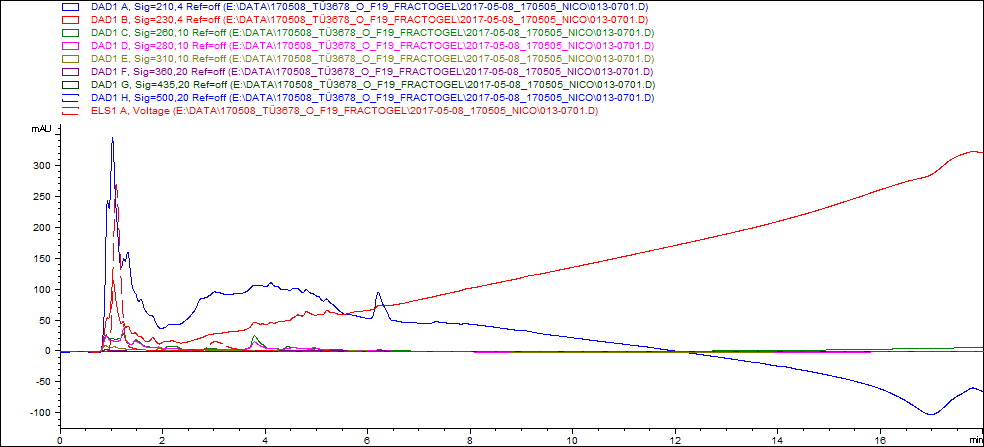
\includegraphics[width=\linewidth]{media_sup_500}
			\caption{NL 500 medium supernatant}
		\end{subfigure}
		\begin{subfigure}{0.8\textwidth}
			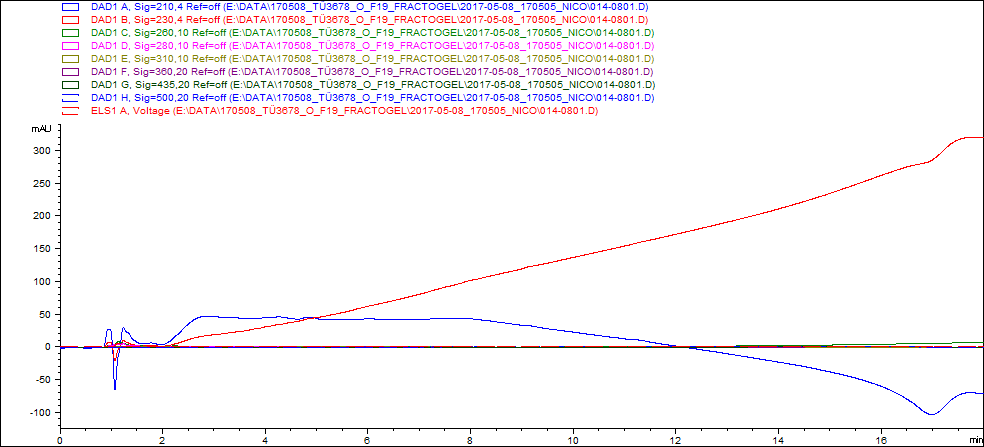
\includegraphics[width=\linewidth]{media_sup_om}
			\caption{OM medium supernatant}
		\end{subfigure}
		\caption[Chromatogram of medium supernatant screening]{\textbf{Chromatogram of medium supernatant screening.} \SI{5}{\micro\liter} of medium supernatant were injected and separated on a C18 column. A screening gradient of 4.5 to 100~\% acetonitril was employed. UV absorption and ELSD voltage were measured.}
		\label{fig:results_medium_screen}
	\end{figure}
	
	The screening chromatograms show, that most compounds in the medium supernatants are rather hydrophilic. No UV absorption or ELSD voltage peaks can be observed after \SI{7}{\minute}. In the case of OM, only one peak is present at the time of injection. The OM supernatant seems to predominantly contain compounds, that can not be separated with a reverse-phase screening gradient on a C18~column. The hydrophilic, antibiotic compound of interest showed no retention under similar conditions. The use of OM as a production medium would therefore lead to fewer impurities in the hydrophobic spectrum. Combined with the visible antibacterial activity of the supernatant against \textit{E. coli}~K12 after only four days and the ease of preparation and filtration, OM was chosen as the default production medium for further experiments.
	
	\subsection{Extraction experiments}
	\label{sub:extraction_experiments}
	
	Three organic solvents, which are immiscible with water, were tested for extraction of the antibiotic compound. Ethyl acetate, methyl acetate and ethyl formate. Additionally, the supernatant was adjusted to five different pH~values ranging from 2 to 11. A hydrophilic molecule is likely to contain functional groups like amines or carboxylic acids, which are charged at certain pH-ranges. If the compound does too, the isoelectric point could passed by pH adjustment. Through reduced charge, the water-solubility could be lowered, enabling the extraction with an organic solvent.
	
	OM medium supernatant was divided into three groups of five aliquots. The pH of each aliquot was adjusted to either 2, 5, 7, 9 or 11. Each group was then extracted with either ethyl acetate, methyl acetate or ethyl formate. Both phases were separated and tested for bioactivity against \coli. 
	
	\begin{figure}[htbp]
		\centering
		\begin{subfigure}{\textwidth}
			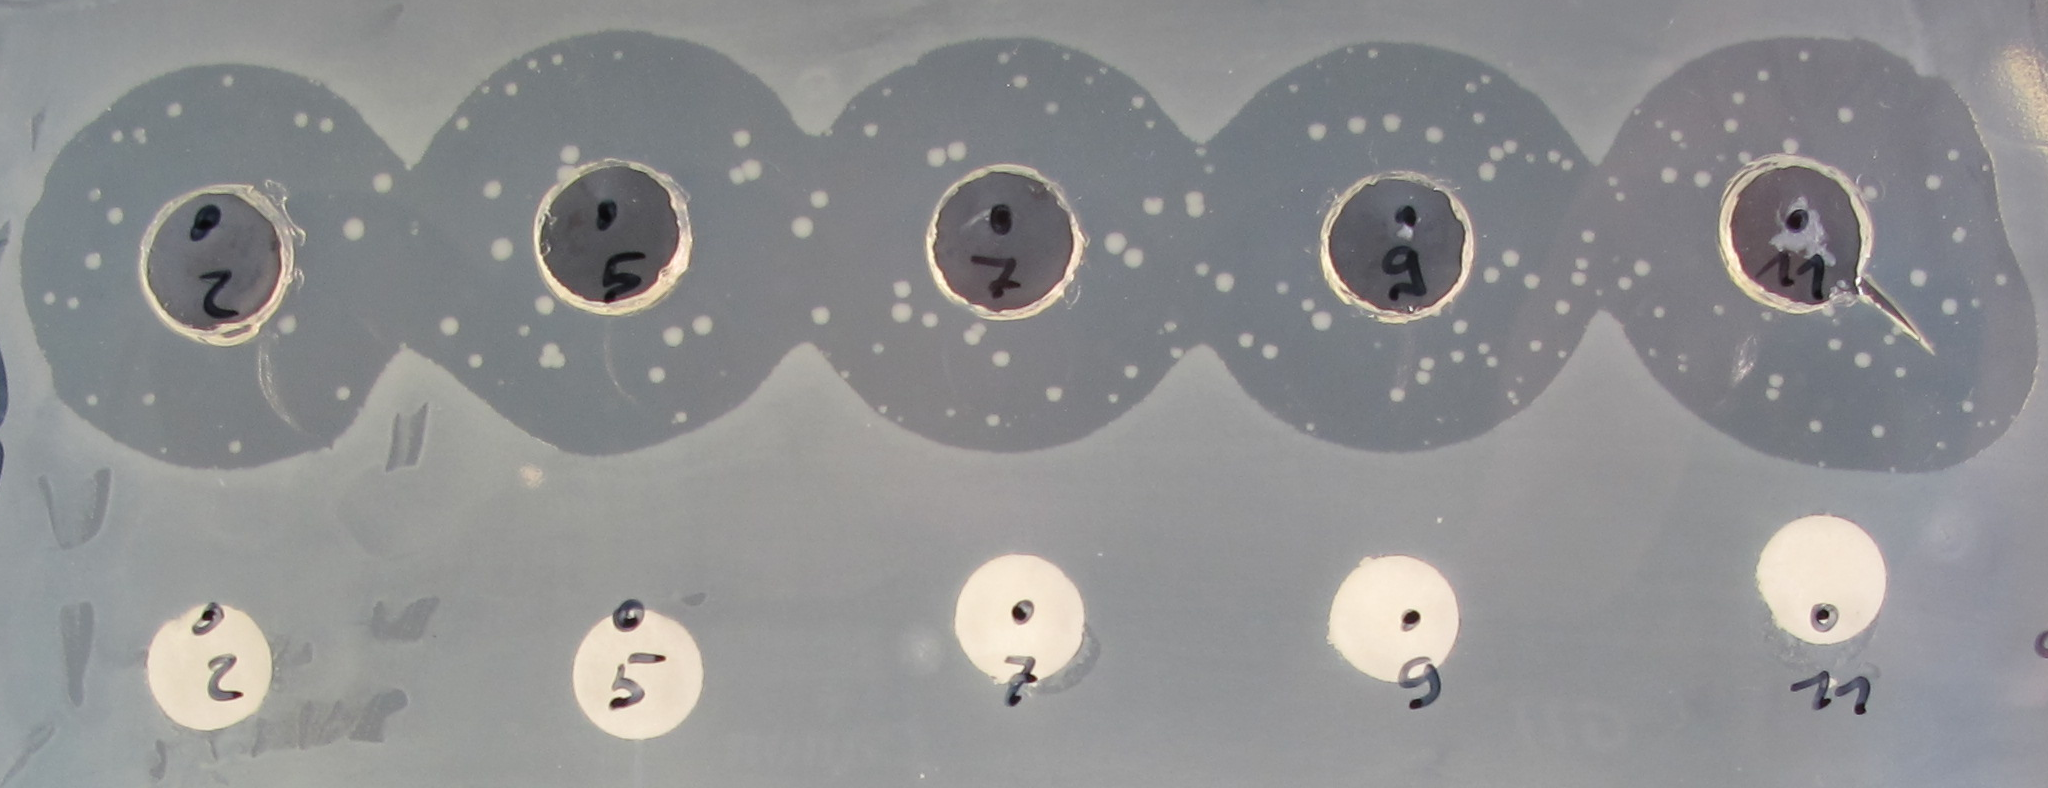
\includegraphics[width=\linewidth]{medium_ph_etac}
			\caption{Ethyl acetate}
		\end{subfigure}
		\begin{subfigure}{\textwidth}
			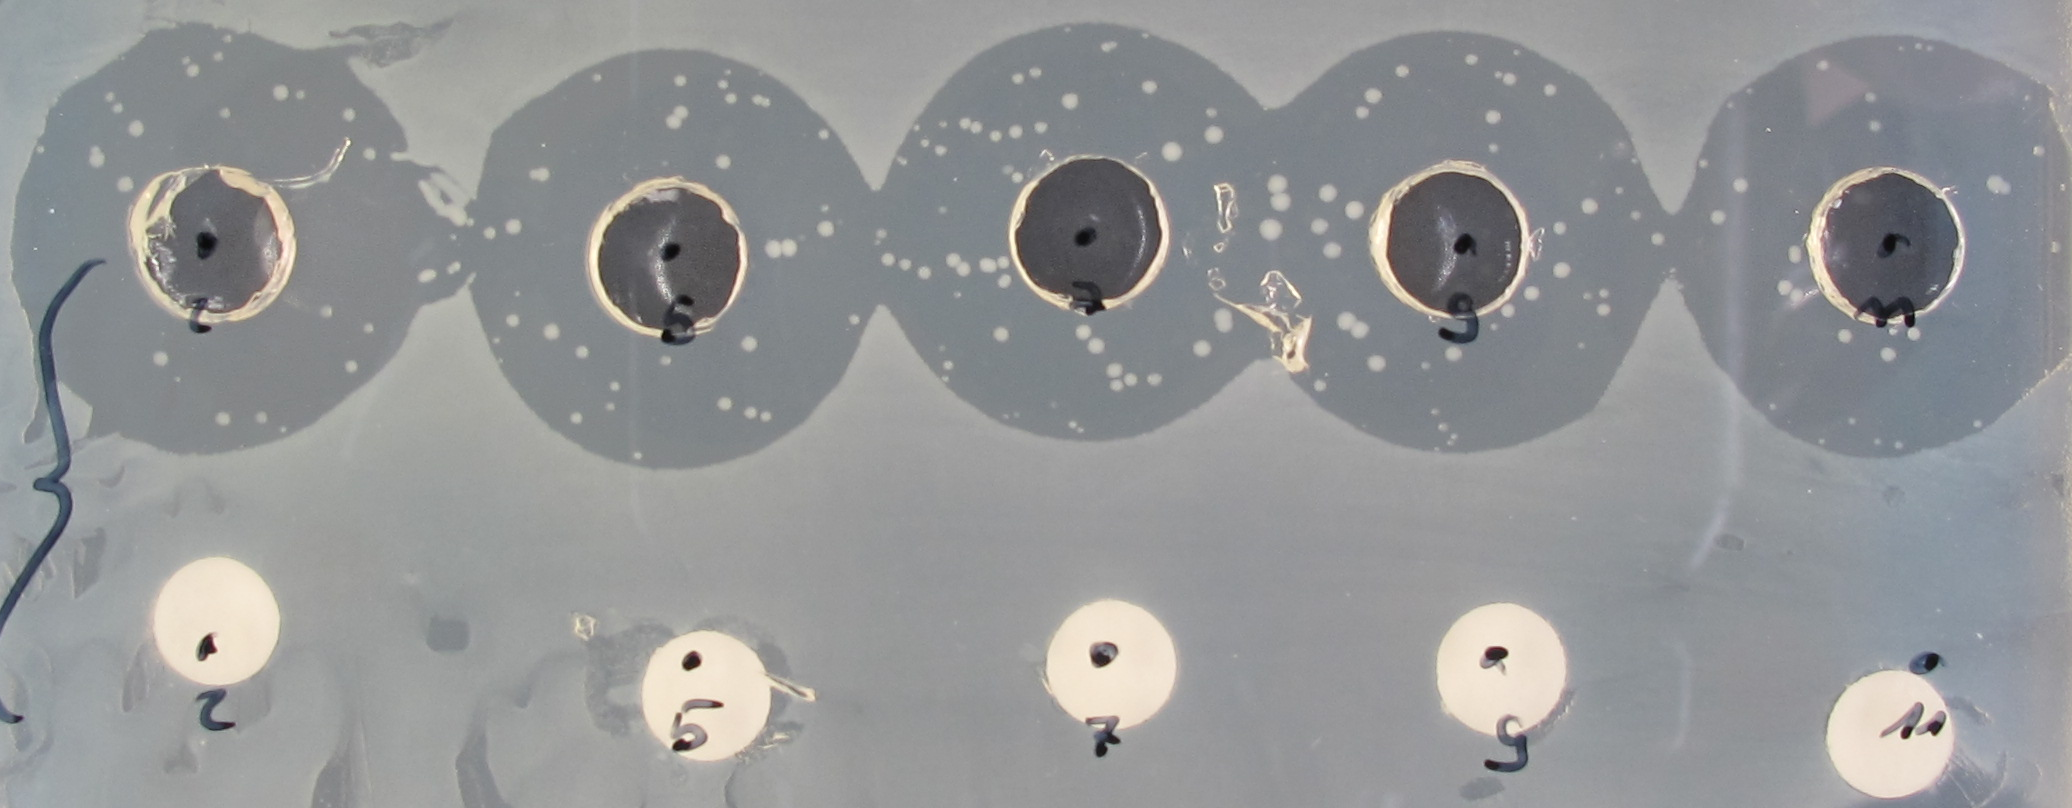
\includegraphics[width=\linewidth]{medium_ph_meac}
			\caption{Methyl acetate}
		\end{subfigure}
		\begin{subfigure}{\textwidth}
			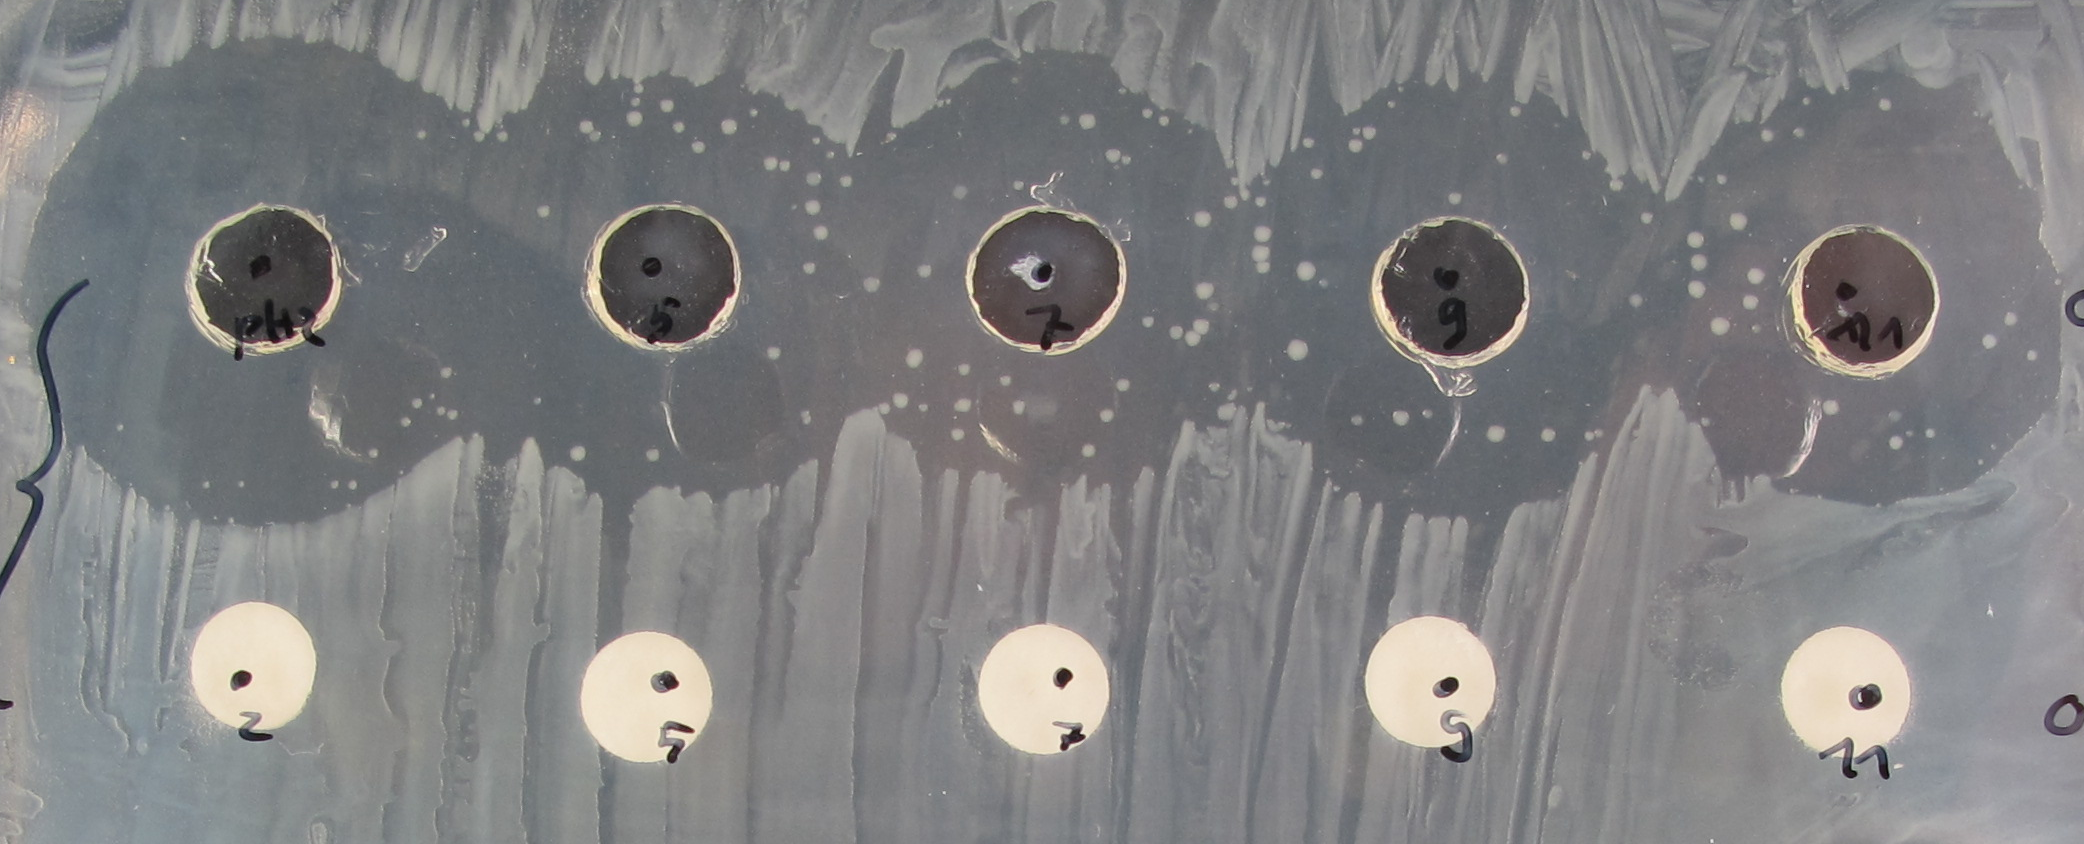
\includegraphics[width=\linewidth]{medium_ph_etform}
			\caption{Ethyl formate}
		\end{subfigure}
		\caption[Bioassay results of different OM medium extracts against \coli]{\textbf{Bioassay results of different OM medium extracts against \coli}}
		\label{fig:results_extraction_bioassay} Filtered supernatant of OM cultures of \tue were extracted with either (a) ethyl acetate, (b) methyl acetate or (c) ethyl formate. Sample-pH was adjusted prior to either 2, 5, 7, 9 or 11 (left to right). Both phases were tested seperately. Upper row consists of \SI{50}{\micro\liter} aqueous phase pipetted directly into wells. Lower row consists of \SI{50}{\micro\liter} organic phase pipetted onto a sterile filter plate, which was placed on the agar.
	\end{figure}
	
	%either zwitterionic -> pH ranges too large
	%many polar, but uncharged groups
	%Chromatogramme von beiden Fraktionen
	%Wieviel konnte durch ausschütteln entfernt werden?
	
% section determination_of_extraction_conditions (end)

\section{Chromatographic Separation} % (fold)
\label{sec:results_chromatographic_separation}

    \subsection{Reverse-Phase HPLC} % (fold)
    \label{sub:results_reverse_phase_hplc}

    % subsection reverse_phase_hplc (end)

    \subsection{Hydrophilic Interaction Liquid Chromatography} % (fold)
    \label{sub:results_hydrophilic_interaction_chromatography}
    
	\begin{itemize}
		\item Short reiteration of HILIC
		\item Characteristics of NH2 column
		\item Characteristics of ZIC-HILIC column
	\end{itemize}

	The \luna by Phenomenex features a silica matrix modified with 3-aminopropyl groups. The used model had a particle size of \SI{3.5}{\micro\meter} and a pore size of 100~\AA. The dimensions were $4.6\times250$~mm.
    
	    \subsubsection{Luna NH\textsubscript{2} Column}
	    
	    Separation via the \luna column was performed with an isocratic method (see \ref{tab:method_nh2_standard}). The mobile phase consisted of 80~\% acetonitrile and 20~\% water at a flow of \SI{2.0}{\milli\liter\per\minute}. Both solvents contained 0.1~\% formic acid as a modifier. \SI{50}{\micro\liter} of filtrated reverse extract at pH~11 were injected and fractions collected every minute. The fractions were subjected to the standard agar-diffusion bioassay against \coli. The chromatogram is shown in 
	    
	    % Bild im Anhang anfügen
	    
	    With this method, the water-soluble compound could be separated from the injection peak. Fractions 5, 6 and 7 produced noticeable zones of inhibition, correlating to elution between 4 and 7~min. With the injection peak eluting at 1.5~min, a relative retention of 2.5 to 5.5 min could be achieved. The majority seems to have eluted between 3.5 and 5.5~min, since the inhibition zones of fractions 6 and 7 were the largest with a diameter of \SI{1.7}{\centi\meter}. Fraction 5 only produced a diameter of \SI{1.2}{\centi\meter}. In the UV-chromatogram, two baseline-separated peaks with distinct spectra were detected in the timeframe correlated to bioactivity. The first was detected at 5~min, the second at 6~min. The UV-spectra  indicate that two bioactive compounds with similar retention times have eluted right between the fraction collector timeframes. A single compound should have resulted in the detection of a rather broad peak with long fronting. However, if the compound does not possess a UV-chromophore, an additional method of detection is needed.

		An evaporative light scattering detector (ELSD) can be used to detect analytes without chromophores, as long as they are less volatile than the solvent.\autocite{Mathews2004,Righezza1988,Mourey1984,Charlesworth1978} The detector can be coupled to a standard HPLC system and provides additional analytical data. To eliminate elution differences between different systems, both the ELSD and the fraction collector were attached to the same system behind the UV-detector. Since ELS-detection is inherently destructive, a splitter was used to divide the flow. One fifth was directed to the ELSD, the rest to the fraction collector. With both 
	    
		% Retention ähnlich wenn pH 11 oder nicht eingestellt (ph8)
		% Könnte bedeuten, dass bei beiden Werten gleich geladen wenn ionenaustausch / adsorption dominierende Kraft
		% Schlechte selektivität durch Sample mit wasser
	    
    % subsection hydrophilic_interaction_chromatography (end)

    \subsection{Ion Exchange Chromatography} % (fold)
    \label{sub:results_ion_exchange_chromatography}

	Water-soluble compounds contain polar functional groups, which at certain pH ranges can even be charged.
	A p\textit{K}\textsubscript{a} value comparison of natural products in the Antibase2008 database revealed, that the majority of entries might be charged at pH~2--11.\autocite{Mansson2010}
	44~\% contained an acidic functionality, 17~\% a basic one, and 9~\% both.

    % subsection ion_exchange_chromatography (end)

    \subsection{Thin-Layer Chromatography} % (fold)
    \label{sub:results_thin_layer_chromatography}

    % subsection thin_layer_chromatography (end)
    
    \subsection{Gel-filtration} % (fold)
    \label{sub:results_gel_filtration}

% section chromatographic_separation (end)

\section{Dereplication} % (fold)
\label{sec:dereplication}

    \subsection{HPLC Mass Spectrometry} % (fold)
    \label{sub:hplc_mass_spectrometry}

    % subsection hplc_mass_spectrometry (end)

    \subsection{Trimethylsilane Derivatization and Gas Chromatography} % (fold)
    \label{sub:trimethylsilane_derivatization_and_gas_chromatography_results}

    % subsection trimethylsilane_derivatization_and_gas_chromatography (end)
    
    %mögliche Detektion falls zucker:

% section dereplication (end)

\section{Antibacterial Activity Spectrum} % (fold)
\label{sec:antibacterial_activity_spectrum}


    \subsection{Activity against \textit{Escherichia coli} K12} % (fold)
    \label{sub:activity_against_e_coli}

    % subsection activity_against_e_coli (end)

    \subsection{Activity against \textit{Bacillus subtilis} 168} % (fold)
    \label{sub:activity_against_b_subtilis}

    % subsection activity_against_b_subtilis (end)

    \subsection{Extraction of yorB-inducing Compound} % (fold)
    \label{sub:extraction_of_yorb_inducing_compound}

    Tü2401 displayed positive results in the yorB-Assay \todo{Referenz einsetzen} when grown on ISP2 plates \todo{Referenz einsetzen}. However, all previously generated samples from liquid cultures only showed antibacterial activity.
    %%%%%%%%%%%%%%
    %Einsetzen:
    %%%%%%%%%%%%%%
    % Absatz über Differenzierung von Streptomyceten
    % Einfluss auf Sekundärmetabolismus
    % Überleitung zu Schlussfolgerung: Evtl zweiter Compound nur auf agar produziert
    %%%%%%%%%%%%%%%
    Three cultivation strategies were developed to induce production of the putative compound 2 (PC2):

    \begin{enumerate}
        \item Standing cultures could allow the formation of aerial mycelium at the medium surface. Thus, enabling the synthesis of PC2 and allowing extraction of the liquid medium. Two \SI{500}{\milli\liter} flasks were each filled with \SI{100}{\milli\liter} of liquid ISP2 medium and inoculated with \SI{1}{\milli\liter} of a one-week old NL~410 shake culture. One flask was sealed with an ordinary aluminium cap (AC), the other one with an air-permeable foam cap (FC). Both flasks were cultivated for four days, before the medium was centrifuged and the supernatant filtrated. \SI{50}{\milli\liter} aliquots of each flask were extracted with either BuOH or EtAc, and both phases were collected seperately. The organic phases were dried at \SI{40}{\celsius} and solved in \SI{1}{\milli\liter} MeOH. Both phases of each flask were subjected to the yorB-Assay.
        \item ISP2 agar plates were previously known to enable synthesis of PC2 and could be extracted with prior breakup. Ten round ISP2 agar plates were inoculated with \SI{100}{\micro\liter} of a one-week old NL~410 shake culture and incubated for four days. One half of the plates was extracted with BuOH, the other half was extracted with EtAc.
        \item ISP2 agar plates could also be prepared with low-melting-point agarose (LMPA). This would allow melting of the plates at lower temperatures. Thus, allowing for easier extraction with reduced risk of thermal decomposition during the process. Six ISP2 LMPA agar plates were inoculated with \SI{100}{\micro\liter} of a week-old NL~410 shake culture and incubated for four days. The plates were then melted at \SI{70}{\celsius} and extracted with BuOH and EtAc.
    \end{enumerate}

    All generated extracts and their respective aqueous phases were tested for bioactivity. The standard bioassay was used to determine the antibiotic activity against \textit{E. coli} K12 and \textit{B. subtilis} 168, and the yorB-Assay was used to test for the mode of action. Additonally, agar stamps of grown ISP2 and ISP2 LMPA plates were tested in the yorB-Assay. A summary of the results is shown in \todo{Tabelle einsetzen}.

    \begin{table}[htbp]
        \caption[Bioassay results from agar-plate and standing culture extraction]{\textbf{Bioassay results from agar-plate and standing culture extraction}.\\
        Samples were screened for antibiotic activity against \textit{E. coli} K12 and \textit{B. subtilis} 168 and for promotor induction in the yorB-Assay.
        Samples from standing cultures with foam cap (FC) or aluminium cap (AC), ISP2 agar plates (ISP2) and ISP2 agar plates with low-melting-point agarose (LMPA). Samples were extracted with butanol (BuOH) or ethyl acetate (EtAc) and tested alongside their respective aqueous phases (aq.). \emph{Legend}: \textbf{-} No activity; \textbf{+ / ++ / +++} antibiotic activity with inhibition zone of 1~/~1.0-1.5~/~>1.5~cm; \textbf{n.e.} result non-evaluable}
        \label{tab:yorB_assay_results}
        \centering
        \begin{tabularx}{\textwidth}{>{\hsize=1.4\hsize}X>{\hsize=.9\hsize}X>{\hsize=.9\hsize}X>{\hsize=.9\hsize}X>{\hsize=.9\hsize}X}
            \toprule
            & \multicolumn{3}{c}{Antibacterial} & positive \\
            \cline{2-4}
            \textbf{Sample} & \textbf{\textit{E. coli}}     & \textbf{\textit{B. subtilis}}  & \textbf{yorB}  & \textbf{yorB}    \\
            \midrule
            FC BuOH         & -     & -     & -     & -    \\
            FC BuOH aq.     & -     & -     & -     & -    \\
            FC EtAc         & -     & +++   & ++    & -    \\
            FC EtAc aq.     & -     & -     & -     & -    \\
            AC BuOH         & -     & -     & -     & -    \\
            AC BuOH aq.     & -     & -     & -     & -    \\
            AC EtAc         & -     & -     & +     & -    \\
            AC EtAc aq.     & -     & -     & -     & -    \\
            \midrule
            ISP2 BuOH       & -     & n.e.  & +++   & -    \\
            ISP2 BuOH aq.   & -     & +     & -     & -    \\
            ISP2 EtAc       & -     & ++    & -     & -    \\
            ISP2 EtAc aq.   & +     & n.e.  & -     & +    \\
            ISP2 plaque     &       &       & ++    & ++   \\
            \midrule
            LMPA BuOH       & +     & n.e.  & +++   & -    \\
            LMPA BuOH aq.   & -     & n.e.  & -     & -    \\
            LMPA EtAc       & -     & n.e.  & +++   & -    \\
            LMPA EtAc aq.   & -     & n.e.  & -     & -    \\
            LMPA plaque     &       &       & -     & -    \\
            \bottomrule
        \end{tabularx}
    \end{table}
    % subsection extraction_of_yorb_inducing_compound (end)

% section antibacterial_activity_spectrum (end)

\section{Species Determination and AntiSMASH Cluster Analysis} % (fold)
\label{sec:species_antismash}

    \subsection{Phylogeny of Strain Tü2401} % (fold)
    \label{sub:phylogeny_of_strain_tue2401}

	\begin{figure}[htbp]
		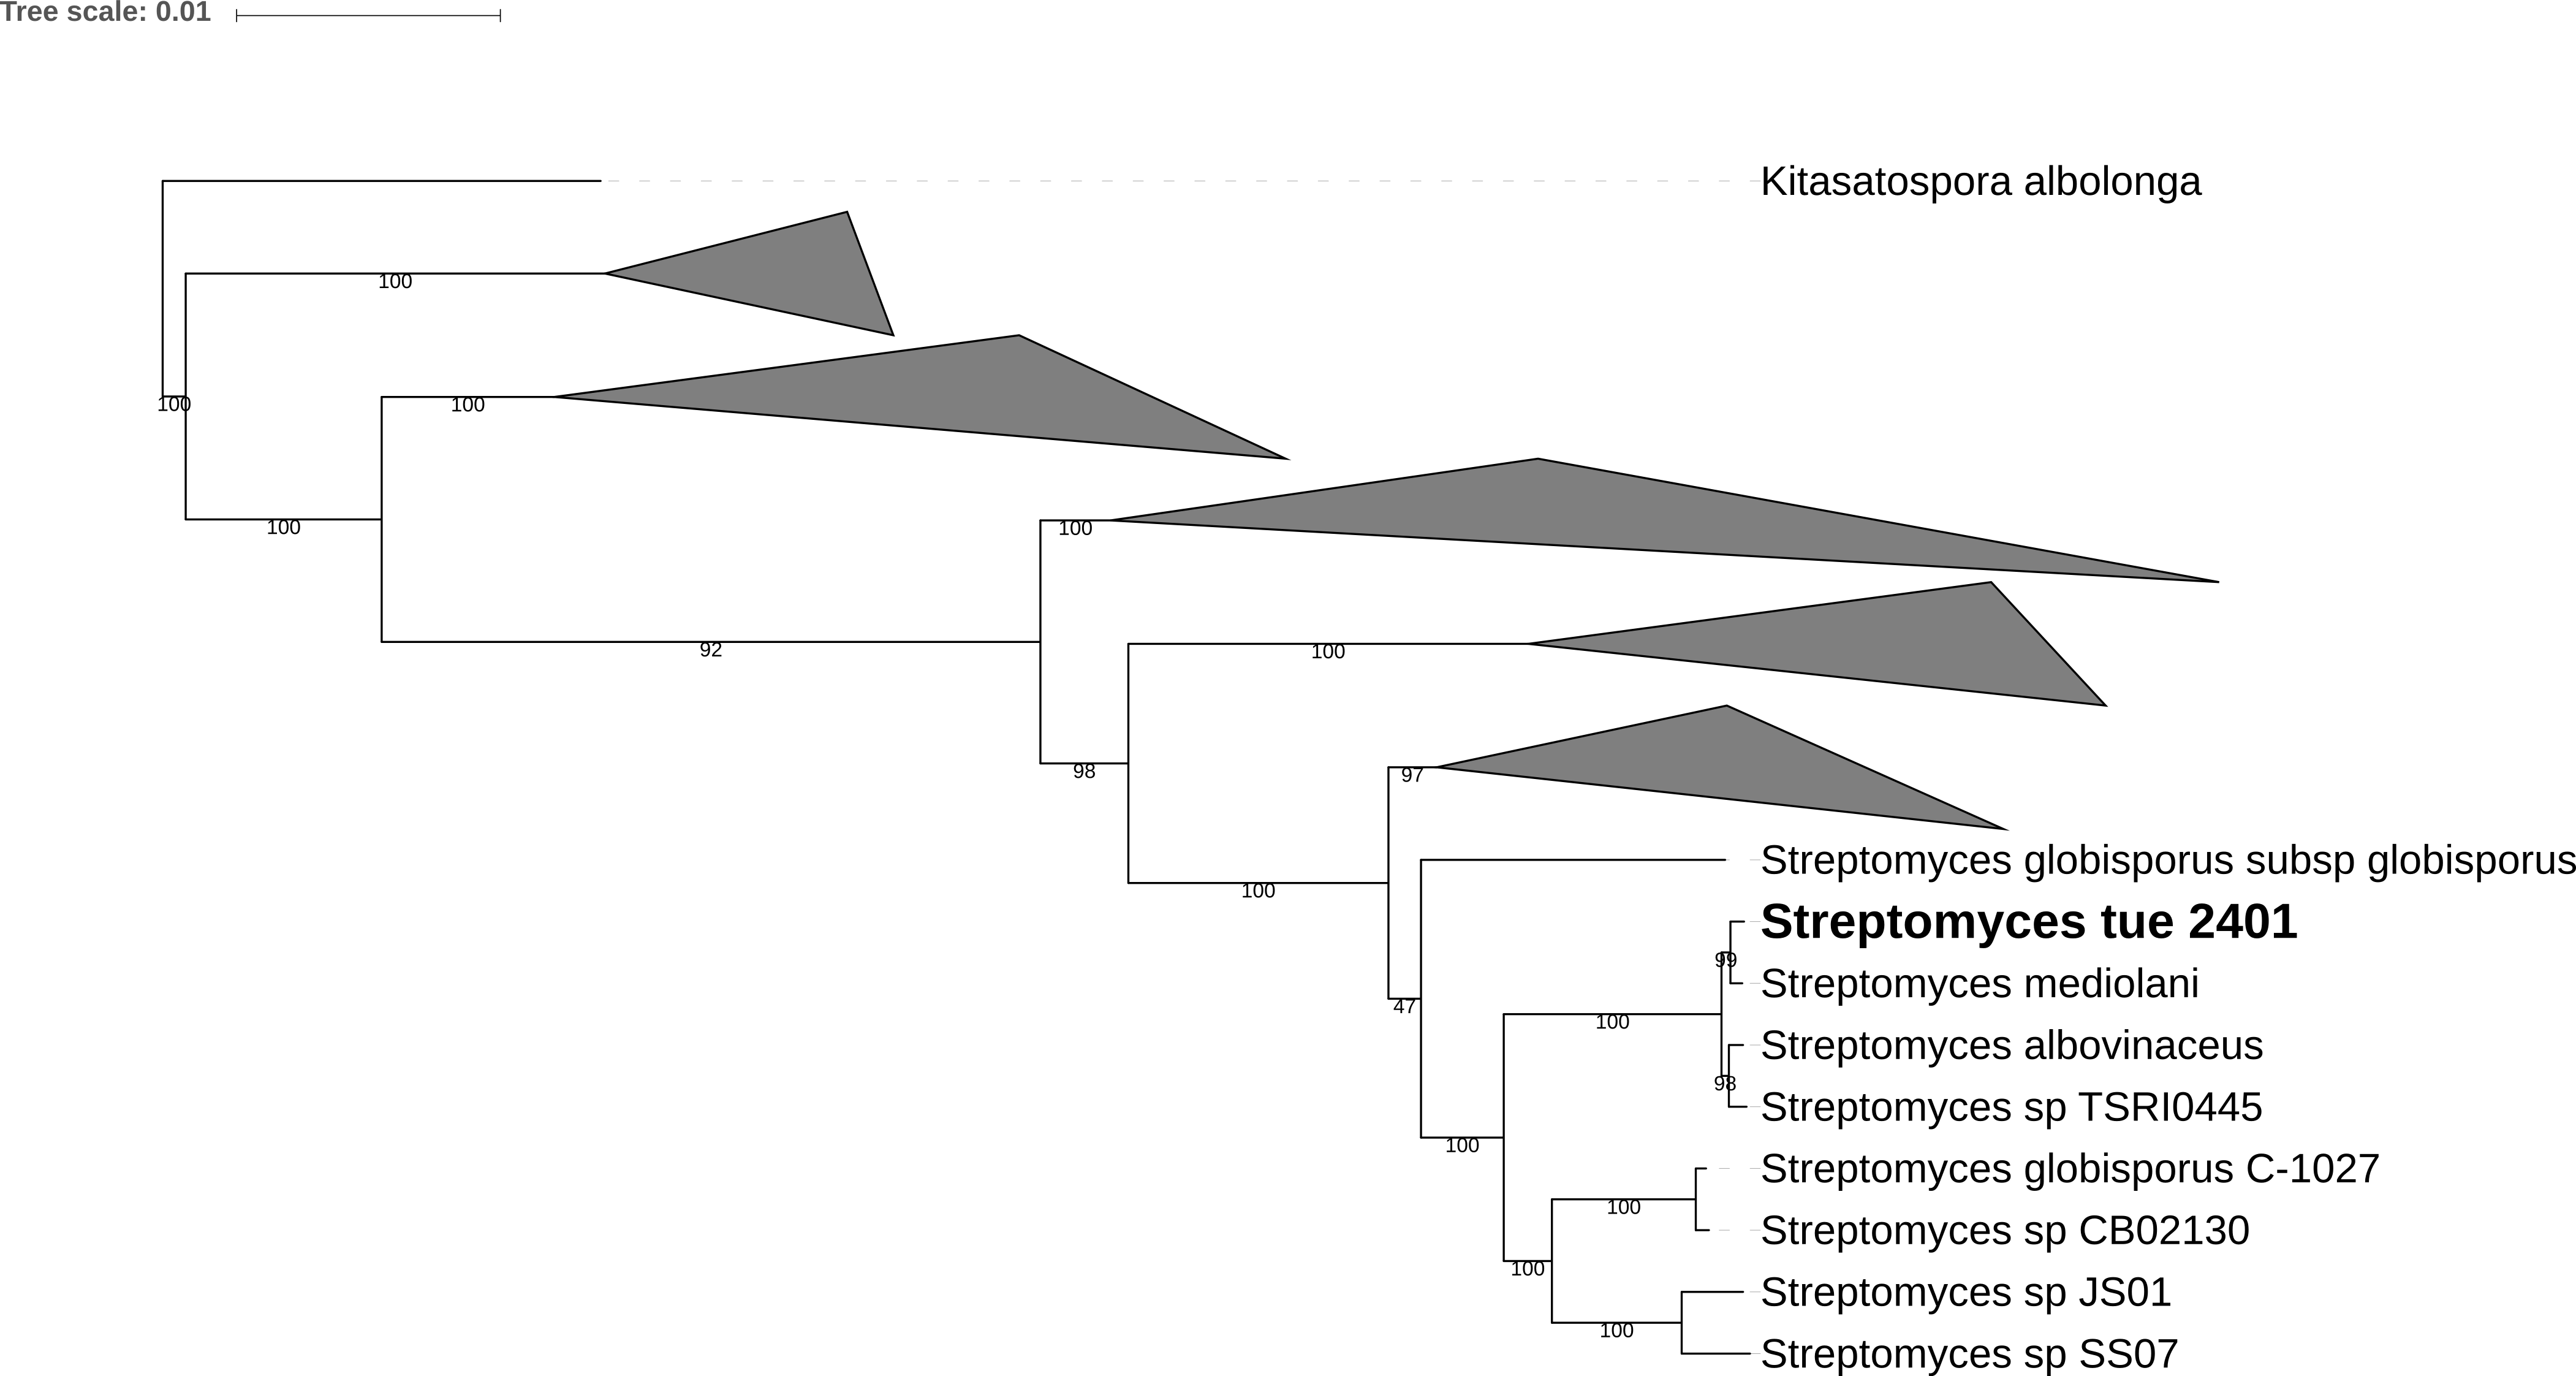
\includegraphics[width=\textwidth]{tu2401_tree}
		\caption[Maximum likelihood tree of \emph{Streptomyces} sp. Tü2401.]{\textbf{Maximum likelihood tree of \emph{Streptomyces} sp. Tü2401.}} The tree was constructed using a multiple-sequence alignment of 50 single-copy genes across 50 \textit{Streptomyces} reference genomes. The node belonging to \textit{Streptomyces}~sp.~Tü2401 is highlighted with bold text. Only the nine most closely related nodes and the outgroup are shown. Dark triangles represented hidden, collapsed nodes.
		\label{fig:phylo_tree} 
	\end{figure}

    % subsection phylogeny_of_strain_tü2401 (end)

    \subsection{AntiSMASH Cluster Identification} % (fold)
    \label{sub:antismash_cluster_identification}

	 One cluster was detected on contig four and identified as a Type1-PKS-NRPS hybrid. It shows a 95~\% cluster identity to the C-1027 biosynthetic gene cluster from \textit{Streptomyces} globisporus C-1027 (MiBiG accession no. BGC0000965). Additionally, three homologous subclusters with 100~\% identity were identified, which are associated with the synthesis of C-1027, Neocarzinostatin and Maduropeptin enediynes (see Figure \ref{fig:cluster_search}).The presence of this cluster could indicate, that the strain Tü2401 is capable of producing a compound similar to enediyne antibiotics. 
	 
	 Enediyne natural products are a class of cytotoxic bacterial compounds, which cause extensive DNA-damage.\autocite{Liang2010,Gredicak2007,AdrianL.Smith*1996,Nicolaou1993} 11 different enediyne natural products are known, all of which feature either a bicyclo[7.3.0]dodecadienediyne core inside a nine-membered ring or a bicyclo[7.3.1]tridecadiynene core inside a ten-membered ring (Figure \ref{fig:enediyne_comparison}). The 9-membered family includes neocarzinostatin, C-1027 and and maduropeptin. The 10-membered family includes calicheamicin $\gamma_{1}^{I}$, esperamicin A\textsubscript{1} and dynemicin A. \autocite{Liang2010} Enediynes are potent cytotoxic agents because of their ability to induce DNA double-strand breaks.\autocite{Shen2015} Electronic rearrangement of the carbocycle produces a benzenoid diradical, which abstracts hydrogen atoms from the DNA-backbone. The consulting radicals cause interstrand crosslinks or react with molecular oxygen.	 
	 \begin{figure}[htbp]
	 	\centering
	 	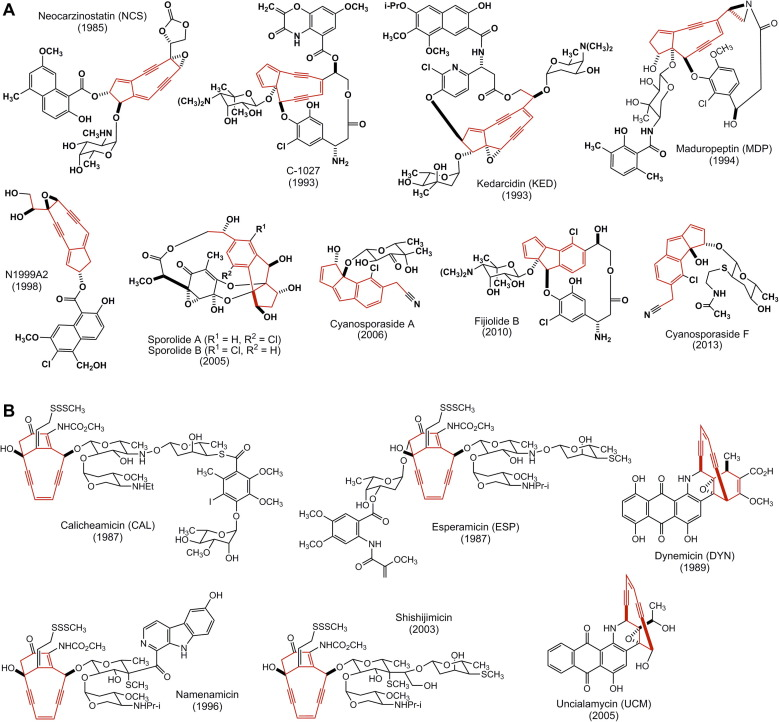
\includegraphics[width=0.9\textwidth]{enediyne_overview}
	 	\caption[Structures of known enediyne natural products]{\textbf{Structures of known enediyne natural products.} Enediyne cores are highlighted in red. (A) Compounds with nine-membered rings. (B) Compounds with ten-membered rings. The year of structure confirmation is displayed in parentheses. The sporolides, cyanosporolids and fijiolides do not contain an endiyene core, but are proposed to be derived from enediyne precursors. Reprinted from Shen \textit{et al.} (2015) Copyright 2014 Elsevier Ltd.}
	 	\label{fig:enediyne_comparison}
	 \end{figure}
	 While the ten-membered enediyne compounds were isolated as free-standing chromophores, most of the compounds in the nine-membered family were isolated in conjunction with a protective apoprotein.\autocite{Liang2010} The nine-membered chromophore of C-1027, which was isolated from \textit{Streptomyces} globisporus C-1027, is bound noncovalently to an 110 amino acid apoprotein.\autocite{AdrianL.Smith*1996,Minami1993,Yoshida1993,Otani1993,Sugiura1993,Matsumoto1993,Otani1991,Otani1988a,Matsumoto1993a} The isolated chromophore has been shown to be very unstable, whereas the holo C-1027 did not lose activity under the same conditions. \autocite{Matsumoto1993,Sugiura1993,Otani1991} The apoprotein binds specifically to the C-1027 chromophore, supposedly by hydrophic pocket, which binds the benzoxazine side chain. \autocite{Okuno1994,Matsumoto1993} The enediyne antibiotics neocarzinostatin and maduropeptin, which were also isolated from actinomycetes, feature highly specific and protective apoproteins as well. \autocite{AdrianL.Smith*1996}.
	 
	 The homologies of the identified cluster could be an indicator, that the strain Tü2401 is capable of synthesizing an enediyene antibiotic with a nine-membered core and a corresponding apoprotein. The potent DNA-strand-breaking capabilities of this compound-class could induce the \textit{yorB} reporter system of \textit{Bacillus subtilis} 1S34 pHJS105-yorB-lacZ2 in the yorB-induction assay. A number of compounds, which cause DNA double strand breaks and crosslinks are reported to induce the system, though none of them belong to the family of endiyne antibiotics. \autocite{Urban2007} Whether this is due to inactivity or to this family not having been tested in the assay is unclear, since the compound library is not publicly accessible. Nevertheless, an endiyne compound could be responsible for the induction.
	 
	 The assay in Section \ref{sub:extraction_of_yorb_inducing_compound} showed, that the \textit{yorB} inducing compound is produced when the strain is grown on an ISP2 agar plate, but it could not be extracted via ethyl acetate or butanol. Only very low activity was retained in the aqueous phase. If the compound is indeed an endiyne, this loss of activity could be due to the high instability of the chromophore. The apoprotein could have been detached during the extraction and concentration process, which also included high temperatures of \SIrange[range-units=single]{40}{60}{\celsius}. Combined with an incubation time of several days between extraction and assay, this could have led to the degradation of the chromophore below the sensitivity threshhold. The high temperatures and long storage times also apply to the numerous HPLC-fractioning samples subjected to the \textit{yorB}-induction assay. 
	 
	 To verify this assumption, the putative endiyne compound has to be extracted by an adapted protocol, dereplicated and subjected to the assay in pure form. The C-1027 antibiotic protein from \textit{S. globisporus} was precipitated from the medium supernatant by the addition of ammonium sulfate and purified by dialysis and column chromatography.\autocite{Otani1988a} The active chromophore could be extracted from the apoprotein with methanol at \SI{0}{\celsius}. \autocite{Matsumoto1993} However, as of now, untreated medium supernatant samples of the strain Tü2401 did not induce the \textit{yorB}-reporter system. The cultivation in liquid OM medium is probably not sufficient for production of the putative endiyene compound and the protocol would have to be adapted for the extraction from ISP2 agar plates. To circumvent this, other cultivation media could be employed and tested for \textit{yorB}-induction. The holo endiyne-apoprotein complex should be stable enough for routine testing of media and media supernatants. The only alternative to optimizing production conditions would be heterologous expression of the biosynthetic cluster. For the endiyne compound family though, this has, as of now, only been partly achieved for the nine-membered endiyne neocarzinostatin.\autocite{Zhang2008}
	 
	 The isolation of the putative endiyne antibiotic would be a very promising target. Only eleven compounds of this class are known to this date, yet several members are in use or development as anticancer drugs with promising results.\autocite{Liang2010,Galm2005} Isolation of a new endiyne compound could  hold a strong promise for the discovery of a new anticancer drug lead structure.
	 
    % subsection antismash_cluster_identification (end)

% section genomic_analysis (end)



% \clearpage

% \printbibliography

\addchap*{Appendix}
% !TEX root = ../main.tex

\chapter{Appendix}

\section*{HPLC Methods} % (fold)
\label{sec:hplc_methods}

	Vielleicht wenn hier text steht

	\begin{table}[htbp]
		\caption[Standard aminocolumn method]{\textbf{Standard Screening Method}}
		\label{tab:method_c18_screening}
		\centering
		\begin{tabularx}{\textwidth}{XX}
			\toprule
			\textbf{Parameter}	& \textbf{Value}	\\
			\midrule
			Column 		& Nucleosil-100 C18 \SI{5}{\micro\meter} 150$\times$\SI{3}{\milli\meter} 	\\
			Solvents	& A: Water + 0.1~\% Formic acid 	\\
						& B: Acetonitrile + 0.1~\% Formic acid		\\
			Method 		& Gradient 5 - 100 \% B for \SI{15}{\minute} 	\\
						& Plateau 100 \% B for \SI{3}{\minute} 	\\
			Flow 		& \SI{1.25}{\milli\liter\per\minute} \\
			Temperature & \SI{25}{\celsius} 	\\
			Injection Volume 	& \SI{50}{\micro\liter} 	\\
			\bottomrule
		\end{tabularx}
	\end{table}

	\begin{table}[htbp]
		\caption[Standard aminocolumn method]{\textbf{Standard aminocolumn method}}
		\label{tab:method_nh2_standard}
		\centering
		\begin{tabularx}{\textwidth}{XX}
			\toprule
			\textbf{Parameter}	& \textbf{Value}	\\
			\midrule
			Column 		& Luna NH2 \SI{5}{\micro\meter} 250$\times$\SI{4.6}{\milli\meter} 	\\
			Solvents	& A: Water + 0.1~\% Formic acid 	\\
						& B: Acetonitrile + 0.1~\% Formic acid		\\
			Method 		& Isocratic 80~\% B for \SI{20}{\minute} 	\\
						& + 100~\% A for \SI{10}{\minute}   \\
			Flow 		& \SI{2}{\milli\liter\per\minute} \\
			Temperature & \SI{25}{\celsius} 	\\
			Injection Volume 	& \SI{50}{\micro\liter} 	\\
			\bottomrule
		\end{tabularx}
	\end{table}

	\begin{table}[htbp]
		\caption[The standard HILIC method]{\textbf{The standard HILIC method}}
		\label{tab:method_hilic_standard}
		\centering
		\begin{tabularx}{\textwidth}{XX}
			\toprule
			\textbf{Component}	& \textbf{Parameter}	\\
			\midrule
			Column 		& ZIC-HILIC \SI{3.5}{\micro\meter} 150$\times$\SI{4.6}{\milli\meter} 	\\
			Solvents	& A: 	10~mM Ammonium acetate 	\\
						& B: 	Acetonitrile 			\\
			Method 		& Isocratic 80~\% B for 45 min. 	\\
			Flow 		& \SI{0.8}{\milli\liter\per\minute} \\
			Temperature & \SI{25}{\celsius} 	\\
			Injection Volume 	& \SI{50}{\micro\liter} 	\\
			\bottomrule
		\end{tabularx}
	\end{table}

	\begin{table}[htbp]
		\caption[Standard aminocolumn method]{\textbf{HILIC method adapted for MS coupling}}
		\label{tab:method_hilic_ms}
		\centering
		\begin{tabularx}{\textwidth}{XX}
			\toprule
			\textbf{Component}	& \textbf{Parameter}	\\
			\midrule
			Column 		& ZIC-HILIC \SI{3.5}{\micro\meter} 150$\times$\SI{4.6}{\milli\meter} 	\\
			Solvents	& A: 	10~mM Ammonium acetate 	\\
						& B: 	Acetonitrile 			\\
			Method 		& Isocratic 80~\% B for 60 min. 	\\
			Flow 		& \SI{0.5}{\milli\liter\per\minute} \\
			Temperature & \SI{40}{\celsius} 	\\
			Injection Volume 	& \SI{50}{\micro\liter} 	\\
			\bottomrule
		\end{tabularx}
	\end{table}

	\begin{table}[htbp]
		\caption[Screening method for HPLC-MS]{\textbf{Screening method for HPLC-MS}}
		\label{tab:method_ms_1}
		\centering
		\begin{tabularx}{\textwidth}{XX}
			\toprule
			\textbf{Parameter}	& \textbf{Value}	\\
			\midrule
			Column 		& Nucleosil-100 \SI{5}{\micro\meter} 150$\times$\SI{3}{\milli\meter} 	\\
			Solvents	& A: Water + 0.1~\% Formic acid 	\\
						& B: Acetonitrile + 0.06~\% Formic acid		\\
			Method 		& Gradient 0 - 100 \% B for \SI{15}{\minute} 	\\
						& Plateau 100 \% B for \SI{2}{\minute} 	\\
			Flow 		& \SI{0.4}{\milli\liter\per\minute} \\
			Temperature & \SI{40}{\celsius} 	\\
			Injection Volume 	& \SI{2.5}{\micro\liter} 	\\
			\midrule
			Capillary Voltage 	& \SI{3500}{\volt} 	\\
			Injector Temperature& \SI{350}{\celsius}\\
			Target mass 		& 400 m/z 			\\
			\bottomrule
		\end{tabularx}
	\end{table}

	\begin{table}[htbp]
		\caption[Screening Method Polar-C18]{\textbf{Screening Method Polar-C18}}
		\label{tab:method_polarc18_screening}
		\centering
		\begin{tabularx}{\textwidth}{XX}
			\toprule
			\textbf{Parameter}	& \textbf{Value}	\\
			\midrule
			Column 		& Kinetex Polar-C18 \SI{2.6}{\micro\meter} 150$\times$\SI{4.6}{\milli\meter} 	\\
			Solvents	& A: Water + 0.1~\% Formic acid 	\\
						& B: Acetonitrile + 0.1~\% Formic acid		\\
			Method 		& Gradient 5 - 100 \% B for \SI{20}{\minute} 	\\
						& Plateau 100 \% B for \SI{6}{\minute} 	\\
			Flow 		& \SI{1.2}{\milli\liter\per\minute} \\
			Temperature & \SI{50}{\celsius} 	\\
			Injection Volume 	& \SI{50}{\micro\liter} 	\\
			\bottomrule
		\end{tabularx}
	\end{table}

	\begin{table}[htbp]
		\caption[Reverse Screening Method Polar-C18]{\textbf{Reverse Screening Method Polar-C18}}
		\label{tab:method_polarc18_revscreening}
		\centering
		\begin{tabularx}{\textwidth}{XX}
			\toprule
			\textbf{Parameter}	& \textbf{Value}	\\
			\midrule
			Column 		& Kinetex Polar-C18 \SI{2.6}{\micro\meter} 150$\times$\SI{4.6}{\milli\meter} 	\\
			Solvents	& A: Water + 0.1~\% Formic acid 	\\
						& B: Acetonitrile + 0.1~\% Formic acid		\\
			Method 		& Gradient 100 - 5 \% B for \SI{20}{\minute} 	\\
						& Plateau 100 \% B for \SI{6}{\minute} 	\\
			Flow 		& \SI{1.2}{\milli\liter\per\minute} \\
			Temperature & \SI{50}{\celsius} 	\\
			Injection Volume 	& \SI{50}{\micro\liter} 	\\
			\bottomrule
		\end{tabularx}
	\end{table}

% section hplc_methods (end)

\section*{Genomic analysis} % (fold)
\label{sec:genomic_analysis}

    \begin{figure}[htpb]
        \centering
        \begin{subfigure}[b]{\textwidth}
            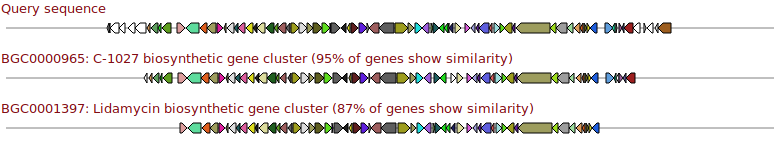
\includegraphics[width=1\linewidth]{contig4_cluster_search}
            \caption{Cluster search results for the identified cluster.}
            \label{fig:sub1}
        \end{subfigure}

        \begin{subfigure}[b]{\textwidth}
            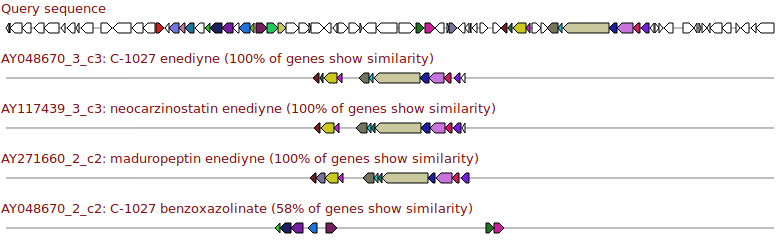
\includegraphics[width=1\linewidth]{contig4_subcluster_search}
            \caption{Subcluster search results for the identified cluster.}
            \label{fig:sub2}
        \end{subfigure}

        \caption[Cluster and subcluster search results for the cluster located on contig four.]{\textbf{Cluster and subcluster search results for the cluster located on contig four.} The 160~kb contig was submitted to AntiSMASH with the ClusterFinder option. Only the search results with the highest similarities are shown.}
        \label{fig:cluster_search}
    \end{figure}

% section genomic_analysis (end)


\end{document}
